% Created by tikzDevice version 0.12.3.1 on 2022-09-05 10:32:52
% !TEX encoding = UTF-8 Unicode
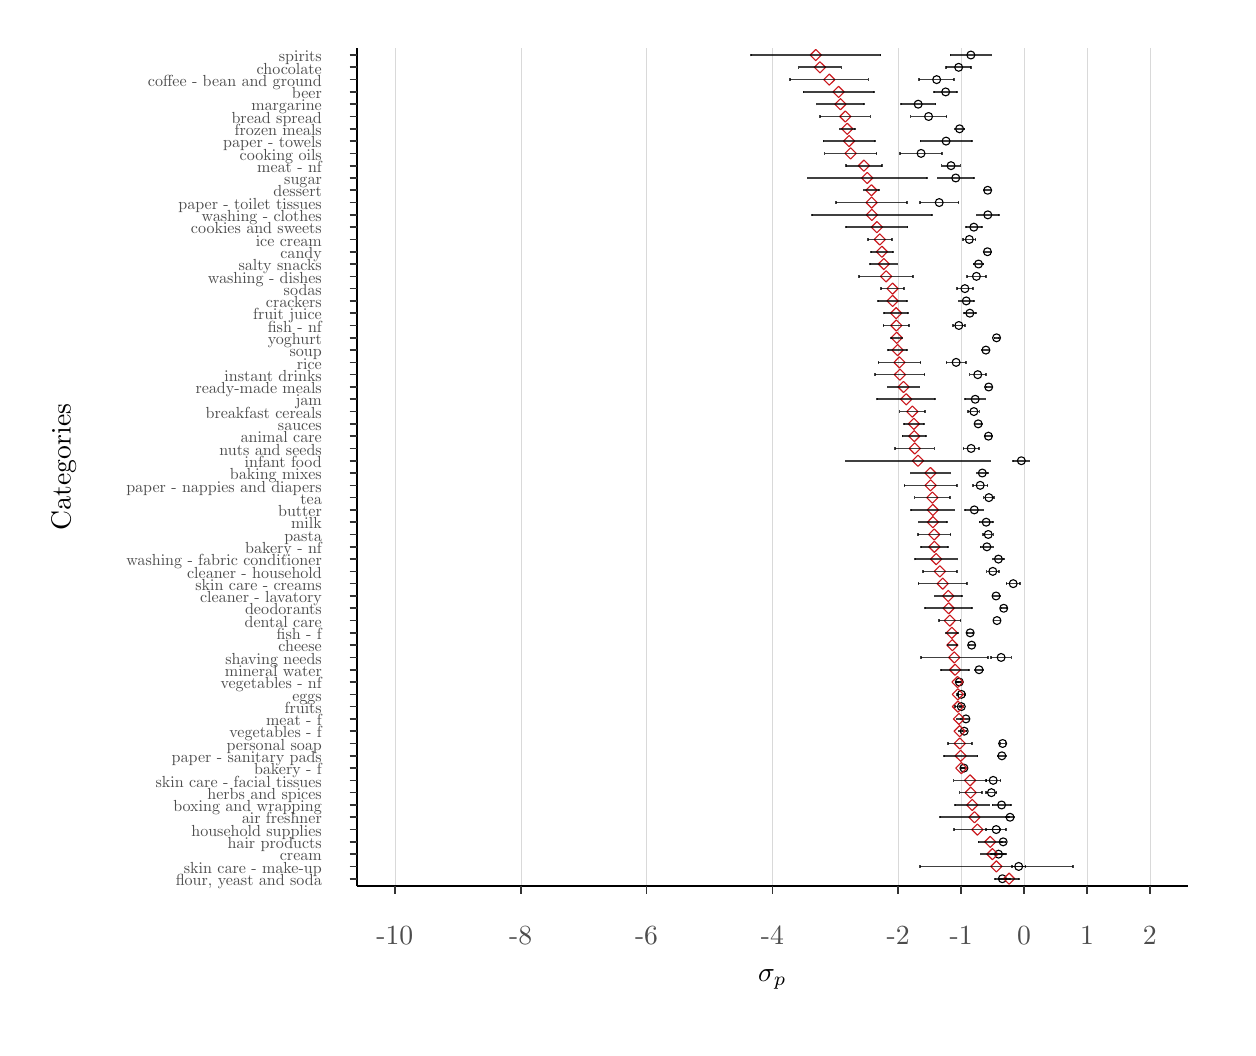
\begin{tikzpicture}[x=1pt,y=1pt]
\definecolor{fillColor}{RGB}{255,255,255}
\path[use as bounding box,fill=fillColor,fill opacity=0.00] (0,0) rectangle (433.62,361.35);
\begin{scope}
\path[clip] (  0.00,  0.00) rectangle (433.62,361.35);
\definecolor{drawColor}{RGB}{255,255,255}
\definecolor{fillColor}{RGB}{255,255,255}

\path[draw=drawColor,line width= 0.6pt,line join=round,line cap=round,fill=fillColor] (  0.00,  0.00) rectangle (433.62,361.35);
\end{scope}
\begin{scope}
\path[clip] (119.04, 51.15) rectangle (419.17,354.12);
\definecolor{drawColor}{RGB}{255,255,255}

\path[draw=drawColor,line width= 0.3pt,line join=round] (155.42, 51.15) --
	(155.42,354.12);

\path[draw=drawColor,line width= 0.3pt,line join=round] (200.89, 51.15) --
	(200.89,354.12);

\path[draw=drawColor,line width= 0.3pt,line join=round] (246.37, 51.15) --
	(246.37,354.12);

\path[draw=drawColor,line width= 0.3pt,line join=round] (291.84, 51.15) --
	(291.84,354.12);

\path[draw=drawColor,line width= 0.3pt,line join=round] (325.95, 51.15) --
	(325.95,354.12);

\path[draw=drawColor,line width= 0.3pt,line join=round] (348.68, 51.15) --
	(348.68,354.12);

\path[draw=drawColor,line width= 0.3pt,line join=round] (371.42, 51.15) --
	(371.42,354.12);

\path[draw=drawColor,line width= 0.3pt,line join=round] (394.16, 51.15) --
	(394.16,354.12);
\definecolor{drawColor}{gray}{0.85}

\path[draw=drawColor,line width= 0.1pt,line join=round] (132.68, 51.15) --
	(132.68,354.12);

\path[draw=drawColor,line width= 0.1pt,line join=round] (178.16, 51.15) --
	(178.16,354.12);

\path[draw=drawColor,line width= 0.1pt,line join=round] (223.63, 51.15) --
	(223.63,354.12);

\path[draw=drawColor,line width= 0.1pt,line join=round] (269.10, 51.15) --
	(269.10,354.12);

\path[draw=drawColor,line width= 0.1pt,line join=round] (314.58, 51.15) --
	(314.58,354.12);

\path[draw=drawColor,line width= 0.1pt,line join=round] (337.31, 51.15) --
	(337.31,354.12);

\path[draw=drawColor,line width= 0.1pt,line join=round] (360.05, 51.15) --
	(360.05,354.12);

\path[draw=drawColor,line width= 0.1pt,line join=round] (382.79, 51.15) --
	(382.79,354.12);

\path[draw=drawColor,line width= 0.1pt,line join=round] (405.52, 51.15) --
	(405.52,354.12);
\definecolor{drawColor}{RGB}{0,0,0}

\path[draw=drawColor,line width= 0.4pt,line join=round,line cap=round] (354.98, 76.03) circle (  1.43);

\path[draw=drawColor,line width= 0.4pt,line join=round,line cap=round] (347.16,213.74) circle (  1.43);

\path[draw=drawColor,line width= 0.4pt,line join=round,line cap=round] (338.31, 93.80) circle (  1.43);

\path[draw=drawColor,line width= 0.4pt,line join=round,line cap=round] (346.61,173.76) circle (  1.43);

\path[draw=drawColor,line width= 0.4pt,line join=round,line cap=round] (344.96,200.42) circle (  1.43);

\path[draw=drawColor,line width= 0.4pt,line join=round,line cap=round] (331.71,338.13) circle (  1.43);

\path[draw=drawColor,line width= 0.4pt,line join=round,line cap=round] (351.92, 80.47) circle (  1.43);

\path[draw=drawColor,line width= 0.4pt,line join=round,line cap=round] (325.54,329.25) circle (  1.43);

\path[draw=drawColor,line width= 0.4pt,line join=round,line cap=round] (341.91,222.63) circle (  1.43);

\path[draw=drawColor,line width= 0.4pt,line join=round,line cap=round] (342.06,187.09) circle (  1.43);

\path[draw=drawColor,line width= 0.4pt,line join=round,line cap=round] (346.81,280.38) circle (  1.43);

\path[draw=drawColor,line width= 0.4pt,line join=round,line cap=round] (341.10,138.22) circle (  1.43);

\path[draw=drawColor,line width= 0.4pt,line join=round,line cap=round] (336.41,347.02) circle (  1.43);

\path[draw=drawColor,line width= 0.4pt,line join=round,line cap=round] (348.75,164.88) circle (  1.43);

\path[draw=drawColor,line width= 0.4pt,line join=round,line cap=round] (349.92,155.99) circle (  1.43);

\path[draw=drawColor,line width= 0.4pt,line join=round,line cap=round] (328.46,342.57) circle (  1.43);

\path[draw=drawColor,line width= 0.4pt,line join=round,line cap=round] (341.89,289.26) circle (  1.43);

\path[draw=drawColor,line width= 0.4pt,line join=round,line cap=round] (322.82,315.92) circle (  1.43);

\path[draw=drawColor,line width= 0.4pt,line join=round,line cap=round] (339.16,262.61) circle (  1.43);

\path[draw=drawColor,line width= 0.4pt,line join=round,line cap=round] (350.81, 62.70) circle (  1.43);

\path[draw=drawColor,line width= 0.4pt,line join=round,line cap=round] (350.25,147.11) circle (  1.43);

\path[draw=drawColor,line width= 0.4pt,line join=round,line cap=round] (352.69,151.55) circle (  1.43);

\path[draw=drawColor,line width= 0.4pt,line join=round,line cap=round] (346.89,302.59) circle (  1.43);

\path[draw=drawColor,line width= 0.4pt,line join=round,line cap=round] (337.38,120.45) circle (  1.43);

\path[draw=drawColor,line width= 0.4pt,line join=round,line cap=round] (340.56,142.67) circle (  1.43);

\path[draw=drawColor,line width= 0.4pt,line join=round,line cap=round] (336.47,253.73) circle (  1.43);

\path[draw=drawColor,line width= 0.4pt,line join=round,line cap=round] (352.20, 53.82) circle (  1.43);

\path[draw=drawColor,line width= 0.4pt,line join=round,line cap=round] (336.73,324.80) circle (  1.43);

\path[draw=drawColor,line width= 0.4pt,line join=round,line cap=round] (340.45,258.17) circle (  1.43);

\path[draw=drawColor,line width= 0.4pt,line join=round,line cap=round] (337.36,116.01) circle (  1.43);

\path[draw=drawColor,line width= 0.4pt,line join=round,line cap=round] (352.49, 67.15) circle (  1.43);

\path[draw=drawColor,line width= 0.4pt,line join=round,line cap=round] (348.24, 84.92) circle (  1.43);

\path[draw=drawColor,line width= 0.4pt,line join=round,line cap=round] (349.97, 71.59) circle (  1.43);

\path[draw=drawColor,line width= 0.4pt,line join=round,line cap=round] (340.26,284.82) circle (  1.43);

\path[draw=drawColor,line width= 0.4pt,line join=round,line cap=round] (359.06,204.86) circle (  1.43);

\path[draw=drawColor,line width= 0.4pt,line join=round,line cap=round] (343.31,235.96) circle (  1.43);

\path[draw=drawColor,line width= 0.4pt,line join=round,line cap=round] (342.39,227.07) circle (  1.43);

\path[draw=drawColor,line width= 0.4pt,line join=round,line cap=round] (321.78,333.69) circle (  1.43);

\path[draw=drawColor,line width= 0.4pt,line join=round,line cap=round] (339.03,111.57) circle (  1.43);

\path[draw=drawColor,line width= 0.4pt,line join=round,line cap=round] (333.65,311.48) circle (  1.43);

\path[draw=drawColor,line width= 0.4pt,line join=round,line cap=round] (346.35,182.65) circle (  1.43);

\path[draw=drawColor,line width= 0.4pt,line join=round,line cap=round] (343.78,129.34) circle (  1.43);

\path[draw=drawColor,line width= 0.4pt,line join=round,line cap=round] (340.91,209.30) circle (  1.43);

\path[draw=drawColor,line width= 0.4pt,line join=round,line cap=round] (344.19,195.97) circle (  1.43);

\path[draw=drawColor,line width= 0.4pt,line join=round,line cap=round] (352.03, 98.24) circle (  1.43);

\path[draw=drawColor,line width= 0.4pt,line join=round,line cap=round] (329.38,298.15) circle (  1.43);

\path[draw=drawColor,line width= 0.4pt,line join=round,line cap=round] (331.86,320.36) circle (  1.43);

\path[draw=drawColor,line width= 0.4pt,line join=round,line cap=round] (347.10,178.21) circle (  1.43);

\path[draw=drawColor,line width= 0.4pt,line join=round,line cap=round] (352.31,102.69) circle (  1.43);

\path[draw=drawColor,line width= 0.4pt,line join=round,line cap=round] (347.26,231.51) circle (  1.43);

\path[draw=drawColor,line width= 0.4pt,line join=round,line cap=round] (335.49,240.40) circle (  1.43);

\path[draw=drawColor,line width= 0.4pt,line join=round,line cap=round] (343.58,275.94) circle (  1.43);

\path[draw=drawColor,line width= 0.4pt,line join=round,line cap=round] (343.46,218.19) circle (  1.43);

\path[draw=drawColor,line width= 0.4pt,line join=round,line cap=round] (351.75,133.78) circle (  1.43);

\path[draw=drawColor,line width= 0.4pt,line join=round,line cap=round] (356.12,160.44) circle (  1.43);

\path[draw=drawColor,line width= 0.4pt,line join=round,line cap=round] (348.88, 89.36) circle (  1.43);

\path[draw=drawColor,line width= 0.4pt,line join=round,line cap=round] (358.10, 58.26) circle (  1.43);

\path[draw=drawColor,line width= 0.4pt,line join=round,line cap=round] (338.67,267.05) circle (  1.43);

\path[draw=drawColor,line width= 0.4pt,line join=round,line cap=round] (346.25,244.84) circle (  1.43);

\path[draw=drawColor,line width= 0.4pt,line join=round,line cap=round] (340.82,351.46) circle (  1.43);

\path[draw=drawColor,line width= 0.4pt,line join=round,line cap=round] (335.35,307.03) circle (  1.43);

\path[draw=drawColor,line width= 0.4pt,line join=round,line cap=round] (347.33,191.53) circle (  1.43);

\path[draw=drawColor,line width= 0.4pt,line join=round,line cap=round] (338.42,107.13) circle (  1.43);

\path[draw=drawColor,line width= 0.4pt,line join=round,line cap=round] (336.64,124.90) circle (  1.43);

\path[draw=drawColor,line width= 0.4pt,line join=round,line cap=round] (346.94,293.71) circle (  1.43);

\path[draw=drawColor,line width= 0.4pt,line join=round,line cap=round] (342.83,271.49) circle (  1.43);

\path[draw=drawColor,line width= 0.4pt,line join=round,line cap=round] (350.78,169.32) circle (  1.43);

\path[draw=drawColor,line width= 0.4pt,line join=round,line cap=round] (350.10,249.28) circle (  1.43);
\definecolor{drawColor}{RGB}{0,0,0}

\path[draw=drawColor,draw opacity=0.75,line width= 0.6pt,line join=round] (356.53, 75.59) --
	(356.53, 76.48);

\path[draw=drawColor,draw opacity=0.75,line width= 0.6pt,line join=round] (356.53, 76.03) --
	(353.44, 76.03);

\path[draw=drawColor,draw opacity=0.75,line width= 0.6pt,line join=round] (353.44, 75.59) --
	(353.44, 76.48);

\path[draw=drawColor,draw opacity=0.75,line width= 0.6pt,line join=round] (348.40,213.30) --
	(348.40,214.19);

\path[draw=drawColor,draw opacity=0.75,line width= 0.6pt,line join=round] (348.40,213.74) --
	(345.92,213.74);

\path[draw=drawColor,draw opacity=0.75,line width= 0.6pt,line join=round] (345.92,213.30) --
	(345.92,214.19);

\path[draw=drawColor,draw opacity=0.75,line width= 0.6pt,line join=round] (338.64, 93.36) --
	(338.64, 94.24);

\path[draw=drawColor,draw opacity=0.75,line width= 0.6pt,line join=round] (338.64, 93.80) --
	(337.98, 93.80);

\path[draw=drawColor,draw opacity=0.75,line width= 0.6pt,line join=round] (337.98, 93.36) --
	(337.98, 94.24);

\path[draw=drawColor,draw opacity=0.75,line width= 0.6pt,line join=round] (348.96,173.32) --
	(348.96,174.21);

\path[draw=drawColor,draw opacity=0.75,line width= 0.6pt,line join=round] (348.96,173.76) --
	(344.27,173.76);

\path[draw=drawColor,draw opacity=0.75,line width= 0.6pt,line join=round] (344.27,173.32) --
	(344.27,174.21);

\path[draw=drawColor,draw opacity=0.75,line width= 0.6pt,line join=round] (347.03,199.97) --
	(347.03,200.86);

\path[draw=drawColor,draw opacity=0.75,line width= 0.6pt,line join=round] (347.03,200.42) --
	(342.88,200.42);

\path[draw=drawColor,draw opacity=0.75,line width= 0.6pt,line join=round] (342.88,199.97) --
	(342.88,200.86);

\path[draw=drawColor,draw opacity=0.75,line width= 0.6pt,line join=round] (335.81,337.69) --
	(335.81,338.57);

\path[draw=drawColor,draw opacity=0.75,line width= 0.6pt,line join=round] (335.81,338.13) --
	(327.61,338.13);

\path[draw=drawColor,draw opacity=0.75,line width= 0.6pt,line join=round] (327.61,337.69) --
	(327.61,338.57);

\path[draw=drawColor,draw opacity=0.75,line width= 0.6pt,line join=round] (355.22, 80.03) --
	(355.22, 80.92);

\path[draw=drawColor,draw opacity=0.75,line width= 0.6pt,line join=round] (355.22, 80.47) --
	(348.62, 80.47);

\path[draw=drawColor,draw opacity=0.75,line width= 0.6pt,line join=round] (348.62, 80.03) --
	(348.62, 80.92);

\path[draw=drawColor,draw opacity=0.75,line width= 0.6pt,line join=round] (332.06,328.80) --
	(332.06,329.69);

\path[draw=drawColor,draw opacity=0.75,line width= 0.6pt,line join=round] (332.06,329.25) --
	(319.03,329.25);

\path[draw=drawColor,draw opacity=0.75,line width= 0.6pt,line join=round] (319.03,328.80) --
	(319.03,329.69);

\path[draw=drawColor,draw opacity=0.75,line width= 0.6pt,line join=round] (343.93,222.18) --
	(343.93,223.07);

\path[draw=drawColor,draw opacity=0.75,line width= 0.6pt,line join=round] (343.93,222.63) --
	(339.88,222.63);

\path[draw=drawColor,draw opacity=0.75,line width= 0.6pt,line join=round] (339.88,222.18) --
	(339.88,223.07);

\path[draw=drawColor,draw opacity=0.75,line width= 0.6pt,line join=round] (345.38,186.65) --
	(345.38,187.53);

\path[draw=drawColor,draw opacity=0.75,line width= 0.6pt,line join=round] (345.38,187.09) --
	(338.73,187.09);

\path[draw=drawColor,draw opacity=0.75,line width= 0.6pt,line join=round] (338.73,186.65) --
	(338.73,187.53);

\path[draw=drawColor,draw opacity=0.75,line width= 0.6pt,line join=round] (348.24,279.94) --
	(348.24,280.82);

\path[draw=drawColor,draw opacity=0.75,line width= 0.6pt,line join=round] (348.24,280.38) --
	(345.38,280.38);

\path[draw=drawColor,draw opacity=0.75,line width= 0.6pt,line join=round] (345.38,279.94) --
	(345.38,280.82);

\path[draw=drawColor,draw opacity=0.75,line width= 0.6pt,line join=round] (342.07,137.78) --
	(342.07,138.67);

\path[draw=drawColor,draw opacity=0.75,line width= 0.6pt,line join=round] (342.07,138.22) --
	(340.14,138.22);

\path[draw=drawColor,draw opacity=0.75,line width= 0.6pt,line join=round] (340.14,137.78) --
	(340.14,138.67);

\path[draw=drawColor,draw opacity=0.75,line width= 0.6pt,line join=round] (340.97,346.57) --
	(340.97,347.46);

\path[draw=drawColor,draw opacity=0.75,line width= 0.6pt,line join=round] (340.97,347.02) --
	(331.85,347.02);

\path[draw=drawColor,draw opacity=0.75,line width= 0.6pt,line join=round] (331.85,346.57) --
	(331.85,347.46);

\path[draw=drawColor,draw opacity=0.75,line width= 0.6pt,line join=round] (351.03,164.43) --
	(351.03,165.32);

\path[draw=drawColor,draw opacity=0.75,line width= 0.6pt,line join=round] (351.03,164.88) --
	(346.48,164.88);

\path[draw=drawColor,draw opacity=0.75,line width= 0.6pt,line join=round] (346.48,164.43) --
	(346.48,165.32);

\path[draw=drawColor,draw opacity=0.75,line width= 0.6pt,line join=round] (351.23,155.55) --
	(351.23,156.44);

\path[draw=drawColor,draw opacity=0.75,line width= 0.6pt,line join=round] (351.23,155.99) --
	(348.60,155.99);

\path[draw=drawColor,draw opacity=0.75,line width= 0.6pt,line join=round] (348.60,155.55) --
	(348.60,156.44);

\path[draw=drawColor,draw opacity=0.75,line width= 0.6pt,line join=round] (334.75,342.13) --
	(334.75,343.02);

\path[draw=drawColor,draw opacity=0.75,line width= 0.6pt,line join=round] (334.75,342.57) --
	(322.17,342.57);

\path[draw=drawColor,draw opacity=0.75,line width= 0.6pt,line join=round] (322.17,342.13) --
	(322.17,343.02);

\path[draw=drawColor,draw opacity=0.75,line width= 0.6pt,line join=round] (344.73,288.82) --
	(344.73,289.71);

\path[draw=drawColor,draw opacity=0.75,line width= 0.6pt,line join=round] (344.73,289.26) --
	(339.05,289.26);

\path[draw=drawColor,draw opacity=0.75,line width= 0.6pt,line join=round] (339.05,288.82) --
	(339.05,289.71);

\path[draw=drawColor,draw opacity=0.75,line width= 0.6pt,line join=round] (330.34,315.47) --
	(330.34,316.36);

\path[draw=drawColor,draw opacity=0.75,line width= 0.6pt,line join=round] (330.34,315.92) --
	(315.30,315.92);

\path[draw=drawColor,draw opacity=0.75,line width= 0.6pt,line join=round] (315.30,315.47) --
	(315.30,316.36);

\path[draw=drawColor,draw opacity=0.75,line width= 0.6pt,line join=round] (341.94,262.17) --
	(341.94,263.05);

\path[draw=drawColor,draw opacity=0.75,line width= 0.6pt,line join=round] (341.94,262.61) --
	(336.37,262.61);

\path[draw=drawColor,draw opacity=0.75,line width= 0.6pt,line join=round] (336.37,262.17) --
	(336.37,263.05);

\path[draw=drawColor,draw opacity=0.75,line width= 0.6pt,line join=round] (353.49, 62.26) --
	(353.49, 63.15);

\path[draw=drawColor,draw opacity=0.75,line width= 0.6pt,line join=round] (353.49, 62.70) --
	(348.13, 62.70);

\path[draw=drawColor,draw opacity=0.75,line width= 0.6pt,line join=round] (348.13, 62.26) --
	(348.13, 63.15);

\path[draw=drawColor,draw opacity=0.75,line width= 0.6pt,line join=round] (351.52,146.66) --
	(351.52,147.55);

\path[draw=drawColor,draw opacity=0.75,line width= 0.6pt,line join=round] (351.52,147.11) --
	(348.99,147.11);

\path[draw=drawColor,draw opacity=0.75,line width= 0.6pt,line join=round] (348.99,146.66) --
	(348.99,147.55);

\path[draw=drawColor,draw opacity=0.75,line width= 0.6pt,line join=round] (353.71,151.11) --
	(353.71,152.00);

\path[draw=drawColor,draw opacity=0.75,line width= 0.6pt,line join=round] (353.71,151.55) --
	(351.66,151.55);

\path[draw=drawColor,draw opacity=0.75,line width= 0.6pt,line join=round] (351.66,151.11) --
	(351.66,152.00);

\path[draw=drawColor,draw opacity=0.75,line width= 0.6pt,line join=round] (348.22,302.15) --
	(348.22,303.04);

\path[draw=drawColor,draw opacity=0.75,line width= 0.6pt,line join=round] (348.22,302.59) --
	(345.55,302.59);

\path[draw=drawColor,draw opacity=0.75,line width= 0.6pt,line join=round] (345.55,302.15) --
	(345.55,303.04);

\path[draw=drawColor,draw opacity=0.75,line width= 0.6pt,line join=round] (338.62,120.01) --
	(338.62,120.90);

\path[draw=drawColor,draw opacity=0.75,line width= 0.6pt,line join=round] (338.62,120.45) --
	(336.14,120.45);

\path[draw=drawColor,draw opacity=0.75,line width= 0.6pt,line join=round] (336.14,120.01) --
	(336.14,120.90);

\path[draw=drawColor,draw opacity=0.75,line width= 0.6pt,line join=round] (341.61,142.22) --
	(341.61,143.11);

\path[draw=drawColor,draw opacity=0.75,line width= 0.6pt,line join=round] (341.61,142.67) --
	(339.51,142.67);

\path[draw=drawColor,draw opacity=0.75,line width= 0.6pt,line join=round] (339.51,142.22) --
	(339.51,143.11);

\path[draw=drawColor,draw opacity=0.75,line width= 0.6pt,line join=round] (338.58,253.28) --
	(338.58,254.17);

\path[draw=drawColor,draw opacity=0.75,line width= 0.6pt,line join=round] (338.58,253.73) --
	(334.37,253.73);

\path[draw=drawColor,draw opacity=0.75,line width= 0.6pt,line join=round] (334.37,253.28) --
	(334.37,254.17);

\path[draw=drawColor,draw opacity=0.75,line width= 0.6pt,line join=round] (354.86, 53.37) --
	(354.86, 54.26);

\path[draw=drawColor,draw opacity=0.75,line width= 0.6pt,line join=round] (354.86, 53.82) --
	(349.53, 53.82);

\path[draw=drawColor,draw opacity=0.75,line width= 0.6pt,line join=round] (349.53, 53.37) --
	(349.53, 54.26);

\path[draw=drawColor,draw opacity=0.75,line width= 0.6pt,line join=round] (338.52,324.36) --
	(338.52,325.25);

\path[draw=drawColor,draw opacity=0.75,line width= 0.6pt,line join=round] (338.52,324.80) --
	(334.94,324.80);

\path[draw=drawColor,draw opacity=0.75,line width= 0.6pt,line join=round] (334.94,324.36) --
	(334.94,325.25);

\path[draw=drawColor,draw opacity=0.75,line width= 0.6pt,line join=round] (342.67,257.72) --
	(342.67,258.61);

\path[draw=drawColor,draw opacity=0.75,line width= 0.6pt,line join=round] (342.67,258.17) --
	(338.22,258.17);

\path[draw=drawColor,draw opacity=0.75,line width= 0.6pt,line join=round] (338.22,257.72) --
	(338.22,258.61);

\path[draw=drawColor,draw opacity=0.75,line width= 0.6pt,line join=round] (337.96,115.57) --
	(337.96,116.46);

\path[draw=drawColor,draw opacity=0.75,line width= 0.6pt,line join=round] (337.96,116.01) --
	(336.77,116.01);

\path[draw=drawColor,draw opacity=0.75,line width= 0.6pt,line join=round] (336.77,115.57) --
	(336.77,116.46);

\path[draw=drawColor,draw opacity=0.75,line width= 0.6pt,line join=round] (353.34, 66.70) --
	(353.34, 67.59);

\path[draw=drawColor,draw opacity=0.75,line width= 0.6pt,line join=round] (353.34, 67.15) --
	(351.64, 67.15);

\path[draw=drawColor,draw opacity=0.75,line width= 0.6pt,line join=round] (351.64, 66.70) --
	(351.64, 67.59);

\path[draw=drawColor,draw opacity=0.75,line width= 0.6pt,line join=round] (350.12, 84.47) --
	(350.12, 85.36);

\path[draw=drawColor,draw opacity=0.75,line width= 0.6pt,line join=round] (350.12, 84.92) --
	(346.36, 84.92);

\path[draw=drawColor,draw opacity=0.75,line width= 0.6pt,line join=round] (346.36, 84.47) --
	(346.36, 85.36);

\path[draw=drawColor,draw opacity=0.75,line width= 0.6pt,line join=round] (353.56, 71.14) --
	(353.56, 72.03);

\path[draw=drawColor,draw opacity=0.75,line width= 0.6pt,line join=round] (353.56, 71.59) --
	(346.38, 71.59);

\path[draw=drawColor,draw opacity=0.75,line width= 0.6pt,line join=round] (346.38, 71.14) --
	(346.38, 72.03);

\path[draw=drawColor,draw opacity=0.75,line width= 0.6pt,line join=round] (342.52,284.38) --
	(342.52,285.27);

\path[draw=drawColor,draw opacity=0.75,line width= 0.6pt,line join=round] (342.52,284.82) --
	(337.99,284.82);

\path[draw=drawColor,draw opacity=0.75,line width= 0.6pt,line join=round] (337.99,284.38) --
	(337.99,285.27);

\path[draw=drawColor,draw opacity=0.75,line width= 0.6pt,line join=round] (361.98,204.42) --
	(361.98,205.30);

\path[draw=drawColor,draw opacity=0.75,line width= 0.6pt,line join=round] (361.98,204.86) --
	(356.15,204.86);

\path[draw=drawColor,draw opacity=0.75,line width= 0.6pt,line join=round] (356.15,204.42) --
	(356.15,205.30);

\path[draw=drawColor,draw opacity=0.75,line width= 0.6pt,line join=round] (346.26,235.51) --
	(346.26,236.40);

\path[draw=drawColor,draw opacity=0.75,line width= 0.6pt,line join=round] (346.26,235.96) --
	(340.37,235.96);

\path[draw=drawColor,draw opacity=0.75,line width= 0.6pt,line join=round] (340.37,235.51) --
	(340.37,236.40);

\path[draw=drawColor,draw opacity=0.75,line width= 0.6pt,line join=round] (346.10,226.63) --
	(346.10,227.52);

\path[draw=drawColor,draw opacity=0.75,line width= 0.6pt,line join=round] (346.10,227.07) --
	(338.67,227.07);

\path[draw=drawColor,draw opacity=0.75,line width= 0.6pt,line join=round] (338.67,226.63) --
	(338.67,227.52);

\path[draw=drawColor,draw opacity=0.75,line width= 0.6pt,line join=round] (328.08,333.24) --
	(328.08,334.13);

\path[draw=drawColor,draw opacity=0.75,line width= 0.6pt,line join=round] (328.08,333.69) --
	(315.49,333.69);

\path[draw=drawColor,draw opacity=0.75,line width= 0.6pt,line join=round] (315.49,333.24) --
	(315.49,334.13);

\path[draw=drawColor,draw opacity=0.75,line width= 0.6pt,line join=round] (339.93,111.13) --
	(339.93,112.01);

\path[draw=drawColor,draw opacity=0.75,line width= 0.6pt,line join=round] (339.93,111.57) --
	(338.14,111.57);

\path[draw=drawColor,draw opacity=0.75,line width= 0.6pt,line join=round] (338.14,111.13) --
	(338.14,112.01);

\path[draw=drawColor,draw opacity=0.75,line width= 0.6pt,line join=round] (337.06,311.03) --
	(337.06,311.92);

\path[draw=drawColor,draw opacity=0.75,line width= 0.6pt,line join=round] (337.06,311.48) --
	(330.23,311.48);

\path[draw=drawColor,draw opacity=0.75,line width= 0.6pt,line join=round] (330.23,311.03) --
	(330.23,311.92);

\path[draw=drawColor,draw opacity=0.75,line width= 0.6pt,line join=round] (348.82,182.20) --
	(348.82,183.09);

\path[draw=drawColor,draw opacity=0.75,line width= 0.6pt,line join=round] (348.82,182.65) --
	(343.88,182.65);

\path[draw=drawColor,draw opacity=0.75,line width= 0.6pt,line join=round] (343.88,182.20) --
	(343.88,183.09);

\path[draw=drawColor,draw opacity=0.75,line width= 0.6pt,line join=round] (345.31,128.90) --
	(345.31,129.78);

\path[draw=drawColor,draw opacity=0.75,line width= 0.6pt,line join=round] (345.31,129.34) --
	(342.24,129.34);

\path[draw=drawColor,draw opacity=0.75,line width= 0.6pt,line join=round] (342.24,128.90) --
	(342.24,129.78);

\path[draw=drawColor,draw opacity=0.75,line width= 0.6pt,line join=round] (343.69,208.86) --
	(343.69,209.75);

\path[draw=drawColor,draw opacity=0.75,line width= 0.6pt,line join=round] (343.69,209.30) --
	(338.14,209.30);

\path[draw=drawColor,draw opacity=0.75,line width= 0.6pt,line join=round] (338.14,208.86) --
	(338.14,209.75);

\path[draw=drawColor,draw opacity=0.75,line width= 0.6pt,line join=round] (346.84,195.53) --
	(346.84,196.42);

\path[draw=drawColor,draw opacity=0.75,line width= 0.6pt,line join=round] (346.84,195.97) --
	(341.54,195.97);

\path[draw=drawColor,draw opacity=0.75,line width= 0.6pt,line join=round] (341.54,195.53) --
	(341.54,196.42);

\path[draw=drawColor,draw opacity=0.75,line width= 0.6pt,line join=round] (353.63, 97.80) --
	(353.63, 98.69);

\path[draw=drawColor,draw opacity=0.75,line width= 0.6pt,line join=round] (353.63, 98.24) --
	(350.43, 98.24);

\path[draw=drawColor,draw opacity=0.75,line width= 0.6pt,line join=round] (350.43, 97.80) --
	(350.43, 98.69);

\path[draw=drawColor,draw opacity=0.75,line width= 0.6pt,line join=round] (336.39,297.70) --
	(336.39,298.59);

\path[draw=drawColor,draw opacity=0.75,line width= 0.6pt,line join=round] (336.39,298.15) --
	(322.38,298.15);

\path[draw=drawColor,draw opacity=0.75,line width= 0.6pt,line join=round] (322.38,297.70) --
	(322.38,298.59);

\path[draw=drawColor,draw opacity=0.75,line width= 0.6pt,line join=round] (341.13,319.92) --
	(341.13,320.81);

\path[draw=drawColor,draw opacity=0.75,line width= 0.6pt,line join=round] (341.13,320.36) --
	(322.59,320.36);

\path[draw=drawColor,draw opacity=0.75,line width= 0.6pt,line join=round] (322.59,319.92) --
	(322.59,320.81);

\path[draw=drawColor,draw opacity=0.75,line width= 0.6pt,line join=round] (348.98,177.76) --
	(348.98,178.65);

\path[draw=drawColor,draw opacity=0.75,line width= 0.6pt,line join=round] (348.98,178.21) --
	(345.21,178.21);

\path[draw=drawColor,draw opacity=0.75,line width= 0.6pt,line join=round] (345.21,177.76) --
	(345.21,178.65);

\path[draw=drawColor,draw opacity=0.75,line width= 0.6pt,line join=round] (353.29,102.24) --
	(353.29,103.13);

\path[draw=drawColor,draw opacity=0.75,line width= 0.6pt,line join=round] (353.29,102.69) --
	(351.33,102.69);

\path[draw=drawColor,draw opacity=0.75,line width= 0.6pt,line join=round] (351.33,102.24) --
	(351.33,103.13);

\path[draw=drawColor,draw opacity=0.75,line width= 0.6pt,line join=round] (348.25,231.07) --
	(348.25,231.96);

\path[draw=drawColor,draw opacity=0.75,line width= 0.6pt,line join=round] (348.25,231.51) --
	(346.27,231.51);

\path[draw=drawColor,draw opacity=0.75,line width= 0.6pt,line join=round] (346.27,231.07) --
	(346.27,231.96);

\path[draw=drawColor,draw opacity=0.75,line width= 0.6pt,line join=round] (339.01,239.95) --
	(339.01,240.84);

\path[draw=drawColor,draw opacity=0.75,line width= 0.6pt,line join=round] (339.01,240.40) --
	(331.97,240.40);

\path[draw=drawColor,draw opacity=0.75,line width= 0.6pt,line join=round] (331.97,239.95) --
	(331.97,240.84);

\path[draw=drawColor,draw opacity=0.75,line width= 0.6pt,line join=round] (345.42,275.49) --
	(345.42,276.38);

\path[draw=drawColor,draw opacity=0.75,line width= 0.6pt,line join=round] (345.42,275.94) --
	(341.73,275.94);

\path[draw=drawColor,draw opacity=0.75,line width= 0.6pt,line join=round] (341.73,275.49) --
	(341.73,276.38);

\path[draw=drawColor,draw opacity=0.75,line width= 0.6pt,line join=round] (344.76,217.74) --
	(344.76,218.63);

\path[draw=drawColor,draw opacity=0.75,line width= 0.6pt,line join=round] (344.76,218.19) --
	(342.17,218.19);

\path[draw=drawColor,draw opacity=0.75,line width= 0.6pt,line join=round] (342.17,217.74) --
	(342.17,218.63);

\path[draw=drawColor,draw opacity=0.75,line width= 0.6pt,line join=round] (355.47,133.34) --
	(355.47,134.23);

\path[draw=drawColor,draw opacity=0.75,line width= 0.6pt,line join=round] (355.47,133.78) --
	(348.03,133.78);

\path[draw=drawColor,draw opacity=0.75,line width= 0.6pt,line join=round] (348.03,133.34) --
	(348.03,134.23);

\path[draw=drawColor,draw opacity=0.75,line width= 0.6pt,line join=round] (358.58,159.99) --
	(358.58,160.88);

\path[draw=drawColor,draw opacity=0.75,line width= 0.6pt,line join=round] (358.58,160.44) --
	(353.67,160.44);

\path[draw=drawColor,draw opacity=0.75,line width= 0.6pt,line join=round] (353.67,159.99) --
	(353.67,160.88);

\path[draw=drawColor,draw opacity=0.75,line width= 0.6pt,line join=round] (351.54, 88.91) --
	(351.54, 89.80);

\path[draw=drawColor,draw opacity=0.75,line width= 0.6pt,line join=round] (351.54, 89.36) --
	(346.22, 89.36);

\path[draw=drawColor,draw opacity=0.75,line width= 0.6pt,line join=round] (346.22, 88.91) --
	(346.22, 89.80);

\path[draw=drawColor,draw opacity=0.75,line width= 0.6pt,line join=round] (360.56, 57.82) --
	(360.56, 58.71);

\path[draw=drawColor,draw opacity=0.75,line width= 0.6pt,line join=round] (360.56, 58.26) --
	(355.64, 58.26);

\path[draw=drawColor,draw opacity=0.75,line width= 0.6pt,line join=round] (355.64, 57.82) --
	(355.64, 58.71);

\path[draw=drawColor,draw opacity=0.75,line width= 0.6pt,line join=round] (341.61,266.61) --
	(341.61,267.50);

\path[draw=drawColor,draw opacity=0.75,line width= 0.6pt,line join=round] (341.61,267.05) --
	(335.74,267.05);

\path[draw=drawColor,draw opacity=0.75,line width= 0.6pt,line join=round] (335.74,266.61) --
	(335.74,267.50);

\path[draw=drawColor,draw opacity=0.75,line width= 0.6pt,line join=round] (347.58,244.40) --
	(347.58,245.29);

\path[draw=drawColor,draw opacity=0.75,line width= 0.6pt,line join=round] (347.58,244.84) --
	(344.93,244.84);

\path[draw=drawColor,draw opacity=0.75,line width= 0.6pt,line join=round] (344.93,244.40) --
	(344.93,245.29);

\path[draw=drawColor,draw opacity=0.75,line width= 0.6pt,line join=round] (348.23,351.01) --
	(348.23,351.90);

\path[draw=drawColor,draw opacity=0.75,line width= 0.6pt,line join=round] (348.23,351.46) --
	(333.41,351.46);

\path[draw=drawColor,draw opacity=0.75,line width= 0.6pt,line join=round] (333.41,351.01) --
	(333.41,351.90);

\path[draw=drawColor,draw opacity=0.75,line width= 0.6pt,line join=round] (341.93,306.59) --
	(341.93,307.48);

\path[draw=drawColor,draw opacity=0.75,line width= 0.6pt,line join=round] (341.93,307.03) --
	(328.78,307.03);

\path[draw=drawColor,draw opacity=0.75,line width= 0.6pt,line join=round] (328.78,306.59) --
	(328.78,307.48);

\path[draw=drawColor,draw opacity=0.75,line width= 0.6pt,line join=round] (349.24,191.09) --
	(349.24,191.98);

\path[draw=drawColor,draw opacity=0.75,line width= 0.6pt,line join=round] (349.24,191.53) --
	(345.41,191.53);

\path[draw=drawColor,draw opacity=0.75,line width= 0.6pt,line join=round] (345.41,191.09) --
	(345.41,191.98);

\path[draw=drawColor,draw opacity=0.75,line width= 0.6pt,line join=round] (339.27,106.68) --
	(339.27,107.57);

\path[draw=drawColor,draw opacity=0.75,line width= 0.6pt,line join=round] (339.27,107.13) --
	(337.56,107.13);

\path[draw=drawColor,draw opacity=0.75,line width= 0.6pt,line join=round] (337.56,106.68) --
	(337.56,107.57);

\path[draw=drawColor,draw opacity=0.75,line width= 0.6pt,line join=round] (337.37,124.45) --
	(337.37,125.34);

\path[draw=drawColor,draw opacity=0.75,line width= 0.6pt,line join=round] (337.37,124.90) --
	(335.91,124.90);

\path[draw=drawColor,draw opacity=0.75,line width= 0.6pt,line join=round] (335.91,124.45) --
	(335.91,125.34);

\path[draw=drawColor,draw opacity=0.75,line width= 0.6pt,line join=round] (350.96,293.26) --
	(350.96,294.15);

\path[draw=drawColor,draw opacity=0.75,line width= 0.6pt,line join=round] (350.96,293.71) --
	(342.91,293.71);

\path[draw=drawColor,draw opacity=0.75,line width= 0.6pt,line join=round] (342.91,293.26) --
	(342.91,294.15);

\path[draw=drawColor,draw opacity=0.75,line width= 0.6pt,line join=round] (346.23,271.05) --
	(346.23,271.94);

\path[draw=drawColor,draw opacity=0.75,line width= 0.6pt,line join=round] (346.23,271.49) --
	(339.42,271.49);

\path[draw=drawColor,draw opacity=0.75,line width= 0.6pt,line join=round] (339.42,271.05) --
	(339.42,271.94);

\path[draw=drawColor,draw opacity=0.75,line width= 0.6pt,line join=round] (352.90,168.88) --
	(352.90,169.76);

\path[draw=drawColor,draw opacity=0.75,line width= 0.6pt,line join=round] (352.90,169.32) --
	(348.66,169.32);

\path[draw=drawColor,draw opacity=0.75,line width= 0.6pt,line join=round] (348.66,168.88) --
	(348.66,169.76);

\path[draw=drawColor,draw opacity=0.75,line width= 0.6pt,line join=round] (350.87,248.84) --
	(350.87,249.73);

\path[draw=drawColor,draw opacity=0.75,line width= 0.6pt,line join=round] (350.87,249.28) --
	(349.33,249.28);

\path[draw=drawColor,draw opacity=0.75,line width= 0.6pt,line join=round] (349.33,248.84) --
	(349.33,249.73);
\definecolor{drawColor}{RGB}{203,24,29}

\path[draw=drawColor,line width= 0.4pt,line join=round,line cap=round] (340.10, 76.03) --
	(342.12, 78.05) --
	(344.13, 76.03) --
	(342.12, 74.01) --
	cycle;

\path[draw=drawColor,line width= 0.4pt,line join=round,line cap=round] (318.35,213.74) --
	(320.37,215.76) --
	(322.38,213.74) --
	(320.37,211.73) --
	cycle;

\path[draw=drawColor,line width= 0.4pt,line join=round,line cap=round] (335.36, 93.80) --
	(337.37, 95.82) --
	(339.39, 93.80) --
	(337.37, 91.78) --
	cycle;

\path[draw=drawColor,line width= 0.4pt,line join=round,line cap=round] (325.62,173.76) --
	(327.64,175.78) --
	(329.66,173.76) --
	(327.64,171.75) --
	cycle;

\path[draw=drawColor,line width= 0.4pt,line join=round,line cap=round] (324.21,200.42) --
	(326.22,202.43) --
	(328.24,200.42) --
	(326.22,198.40) --
	cycle;

\path[draw=drawColor,line width= 0.4pt,line join=round,line cap=round] (290.99,338.13) --
	(293.01,340.15) --
	(295.03,338.13) --
	(293.01,336.11) --
	cycle;

\path[draw=drawColor,line width= 0.4pt,line join=round,line cap=round] (339.30, 80.47) --
	(341.31, 82.49) --
	(343.33, 80.47) --
	(341.31, 78.46) --
	cycle;

\path[draw=drawColor,line width= 0.4pt,line join=round,line cap=round] (293.43,329.25) --
	(295.45,331.26) --
	(297.46,329.25) --
	(295.45,327.23) --
	cycle;

\path[draw=drawColor,line width= 0.4pt,line join=round,line cap=round] (317.66,222.63) --
	(319.67,224.65) --
	(321.69,222.63) --
	(319.67,220.61) --
	cycle;

\path[draw=drawColor,line width= 0.4pt,line join=round,line cap=round] (325.05,187.09) --
	(327.07,189.11) --
	(329.09,187.09) --
	(327.07,185.07) --
	cycle;

\path[draw=drawColor,line width= 0.4pt,line join=round,line cap=round] (306.65,280.38) --
	(308.67,282.40) --
	(310.68,280.38) --
	(308.67,278.36) --
	cycle;

\path[draw=drawColor,line width= 0.4pt,line join=round,line cap=round] (332.11,138.22) --
	(334.12,140.24) --
	(336.14,138.22) --
	(334.12,136.21) --
	cycle;

\path[draw=drawColor,line width= 0.4pt,line join=round,line cap=round] (284.27,347.02) --
	(286.29,349.03) --
	(288.31,347.02) --
	(286.29,345.00) --
	cycle;

\path[draw=drawColor,line width= 0.4pt,line join=round,line cap=round] (327.61,164.88) --
	(329.63,166.90) --
	(331.64,164.88) --
	(329.63,162.86) --
	cycle;

\path[draw=drawColor,line width= 0.4pt,line join=round,line cap=round] (330.63,155.99) --
	(332.65,158.01) --
	(334.67,155.99) --
	(332.65,153.98) --
	cycle;

\path[draw=drawColor,line width= 0.4pt,line join=round,line cap=round] (287.63,342.57) --
	(289.65,344.59) --
	(291.67,342.57) --
	(289.65,340.56) --
	cycle;

\path[draw=drawColor,line width= 0.4pt,line join=round,line cap=round] (304.86,289.26) --
	(306.88,291.28) --
	(308.90,289.26) --
	(306.88,287.25) --
	cycle;

\path[draw=drawColor,line width= 0.4pt,line join=round,line cap=round] (295.35,315.92) --
	(297.36,317.94) --
	(299.38,315.92) --
	(297.36,313.90) --
	cycle;

\path[draw=drawColor,line width= 0.4pt,line join=round,line cap=round] (310.50,262.61) --
	(312.52,264.63) --
	(314.54,262.61) --
	(312.52,260.59) --
	cycle;

\path[draw=drawColor,line width= 0.4pt,line join=round,line cap=round] (346.60, 62.70) --
	(348.62, 64.72) --
	(350.64, 62.70) --
	(348.62, 60.69) --
	cycle;

\path[draw=drawColor,line width= 0.4pt,line join=round,line cap=round] (331.20,147.11) --
	(333.22,149.13) --
	(335.23,147.11) --
	(333.22,145.09) --
	cycle;

\path[draw=drawColor,line width= 0.4pt,line join=round,line cap=round] (330.77,151.55) --
	(332.79,153.57) --
	(334.81,151.55) --
	(332.79,149.53) --
	cycle;

\path[draw=drawColor,line width= 0.4pt,line join=round,line cap=round] (302.86,302.59) --
	(304.88,304.61) --
	(306.90,302.59) --
	(304.88,300.57) --
	cycle;

\path[draw=drawColor,line width= 0.4pt,line join=round,line cap=round] (334.10,120.45) --
	(336.11,122.47) --
	(338.13,120.45) --
	(336.11,118.44) --
	cycle;

\path[draw=drawColor,line width= 0.4pt,line join=round,line cap=round] (331.92,142.67) --
	(333.94,144.68) --
	(335.96,142.67) --
	(333.94,140.65) --
	cycle;

\path[draw=drawColor,line width= 0.4pt,line join=round,line cap=round] (311.87,253.73) --
	(313.89,255.74) --
	(315.91,253.73) --
	(313.89,251.71) --
	cycle;

\path[draw=drawColor,line width= 0.4pt,line join=round,line cap=round] (352.62, 53.82) --
	(354.64, 55.84) --
	(356.66, 53.82) --
	(354.64, 51.80) --
	cycle;

\path[draw=drawColor,line width= 0.4pt,line join=round,line cap=round] (294.12,324.80) --
	(296.14,326.82) --
	(298.16,324.80) --
	(296.14,322.79) --
	cycle;

\path[draw=drawColor,line width= 0.4pt,line join=round,line cap=round] (311.80,258.17) --
	(313.81,260.19) --
	(315.83,258.17) --
	(313.81,256.15) --
	cycle;

\path[draw=drawColor,line width= 0.4pt,line join=round,line cap=round] (334.14,116.01) --
	(336.16,118.03) --
	(338.18,116.01) --
	(336.16,113.99) --
	cycle;

\path[draw=drawColor,line width= 0.4pt,line join=round,line cap=round] (345.79, 67.15) --
	(347.81, 69.16) --
	(349.82, 67.15) --
	(347.81, 65.13) --
	cycle;

\path[draw=drawColor,line width= 0.4pt,line join=round,line cap=round] (338.73, 84.92) --
	(340.75, 86.93) --
	(342.77, 84.92) --
	(340.75, 82.90) --
	cycle;

\path[draw=drawColor,line width= 0.4pt,line join=round,line cap=round] (341.16, 71.59) --
	(343.18, 73.61) --
	(345.19, 71.59) --
	(343.18, 69.57) --
	cycle;

\path[draw=drawColor,line width= 0.4pt,line join=round,line cap=round] (305.89,284.82) --
	(307.91,286.84) --
	(309.92,284.82) --
	(307.91,282.80) --
	cycle;

\path[draw=drawColor,line width= 0.4pt,line join=round,line cap=round] (319.71,204.86) --
	(321.73,206.88) --
	(323.75,204.86) --
	(321.73,202.84) --
	cycle;

\path[draw=drawColor,line width= 0.4pt,line join=round,line cap=round] (313.17,235.96) --
	(315.19,237.97) --
	(317.21,235.96) --
	(315.19,233.94) --
	cycle;

\path[draw=drawColor,line width= 0.4pt,line join=round,line cap=round] (315.43,227.07) --
	(317.45,229.09) --
	(319.47,227.07) --
	(317.45,225.05) --
	cycle;

\path[draw=drawColor,line width= 0.4pt,line join=round,line cap=round] (291.67,333.69) --
	(293.69,335.71) --
	(295.71,333.69) --
	(293.69,331.67) --
	cycle;

\path[draw=drawColor,line width= 0.4pt,line join=round,line cap=round] (334.50,111.57) --
	(336.52,113.59) --
	(338.53,111.57) --
	(336.52,109.55) --
	cycle;

\path[draw=drawColor,line width= 0.4pt,line join=round,line cap=round] (300.15,311.48) --
	(302.17,313.49) --
	(304.19,311.48) --
	(302.17,309.46) --
	cycle;

\path[draw=drawColor,line width= 0.4pt,line join=round,line cap=round] (325.09,182.65) --
	(327.10,184.67) --
	(329.12,182.65) --
	(327.10,180.63) --
	cycle;

\path[draw=drawColor,line width= 0.4pt,line join=round,line cap=round] (333.10,129.34) --
	(335.12,131.36) --
	(337.14,129.34) --
	(335.12,127.32) --
	cycle;

\path[draw=drawColor,line width= 0.4pt,line join=round,line cap=round] (318.53,209.30) --
	(320.55,211.32) --
	(322.57,209.30) --
	(320.55,207.28) --
	cycle;

\path[draw=drawColor,line width= 0.4pt,line join=round,line cap=round] (324.23,195.97) --
	(326.25,197.99) --
	(328.27,195.97) --
	(326.25,193.96) --
	cycle;

\path[draw=drawColor,line width= 0.4pt,line join=round,line cap=round] (335.11, 98.24) --
	(337.13,100.26) --
	(339.15, 98.24) --
	(337.13, 96.23) --
	cycle;

\path[draw=drawColor,line width= 0.4pt,line join=round,line cap=round] (302.94,298.15) --
	(304.96,300.17) --
	(306.97,298.15) --
	(304.96,296.13) --
	cycle;

\path[draw=drawColor,line width= 0.4pt,line join=round,line cap=round] (294.79,320.36) --
	(296.81,322.38) --
	(298.82,320.36) --
	(296.81,318.34) --
	cycle;

\path[draw=drawColor,line width= 0.4pt,line join=round,line cap=round] (325.54,178.21) --
	(327.56,180.22) --
	(329.58,178.21) --
	(327.56,176.19) --
	cycle;

\path[draw=drawColor,line width= 0.4pt,line join=round,line cap=round] (334.80,102.69) --
	(336.82,104.70) --
	(338.83,102.69) --
	(336.82,100.67) --
	cycle;

\path[draw=drawColor,line width= 0.4pt,line join=round,line cap=round] (314.47,231.51) --
	(316.49,233.53) --
	(318.50,231.51) --
	(316.49,229.50) --
	cycle;

\path[draw=drawColor,line width= 0.4pt,line join=round,line cap=round] (313.01,240.40) --
	(315.02,242.42) --
	(317.04,240.40) --
	(315.02,238.38) --
	cycle;

\path[draw=drawColor,line width= 0.4pt,line join=round,line cap=round] (307.35,275.94) --
	(309.37,277.95) --
	(311.39,275.94) --
	(309.37,273.92) --
	cycle;

\path[draw=drawColor,line width= 0.4pt,line join=round,line cap=round] (318.20,218.19) --
	(320.21,220.20) --
	(322.23,218.19) --
	(320.21,216.17) --
	cycle;

\path[draw=drawColor,line width= 0.4pt,line join=round,line cap=round] (332.81,133.78) --
	(334.83,135.80) --
	(336.85,133.78) --
	(334.83,131.76) --
	cycle;

\path[draw=drawColor,line width= 0.4pt,line join=round,line cap=round] (328.63,160.44) --
	(330.65,162.45) --
	(332.66,160.44) --
	(330.65,158.42) --
	cycle;

\path[draw=drawColor,line width= 0.4pt,line join=round,line cap=round] (338.51, 89.36) --
	(340.52, 91.38) --
	(342.54, 89.36) --
	(340.52, 87.34) --
	cycle;

\path[draw=drawColor,line width= 0.4pt,line join=round,line cap=round] (348.02, 58.26) --
	(350.04, 60.28) --
	(352.05, 58.26) --
	(350.04, 56.24) --
	cycle;

\path[draw=drawColor,line width= 0.4pt,line join=round,line cap=round] (310.49,267.05) --
	(312.51,269.07) --
	(314.53,267.05) --
	(312.51,265.04) --
	cycle;

\path[draw=drawColor,line width= 0.4pt,line join=round,line cap=round] (312.32,244.84) --
	(314.33,246.86) --
	(316.35,244.84) --
	(314.33,242.82) --
	cycle;

\path[draw=drawColor,line width= 0.4pt,line join=round,line cap=round] (282.77,351.46) --
	(284.79,353.48) --
	(286.80,351.46) --
	(284.79,349.44) --
	cycle;

\path[draw=drawColor,line width= 0.4pt,line join=round,line cap=round] (301.35,307.03) --
	(303.36,309.05) --
	(305.38,307.03) --
	(303.36,305.02) --
	cycle;

\path[draw=drawColor,line width= 0.4pt,line join=round,line cap=round] (324.90,191.53) --
	(326.92,193.55) --
	(328.93,191.53) --
	(326.92,189.51) --
	cycle;

\path[draw=drawColor,line width= 0.4pt,line join=round,line cap=round] (334.74,107.13) --
	(336.76,109.14) --
	(338.77,107.13) --
	(336.76,105.11) --
	cycle;

\path[draw=drawColor,line width= 0.4pt,line join=round,line cap=round] (333.98,124.90) --
	(336.00,126.91) --
	(338.02,124.90) --
	(336.00,122.88) --
	cycle;

\path[draw=drawColor,line width= 0.4pt,line join=round,line cap=round] (303.04,293.71) --
	(305.05,295.72) --
	(307.07,293.71) --
	(305.05,291.69) --
	cycle;

\path[draw=drawColor,line width= 0.4pt,line join=round,line cap=round] (308.17,271.49) --
	(310.19,273.51) --
	(312.21,271.49) --
	(310.19,269.48) --
	cycle;

\path[draw=drawColor,line width= 0.4pt,line join=round,line cap=round] (326.27,169.32) --
	(328.29,171.34) --
	(330.31,169.32) --
	(328.29,167.30) --
	cycle;

\path[draw=drawColor,line width= 0.4pt,line join=round,line cap=round] (312.01,249.28) --
	(314.03,251.30) --
	(316.05,249.28) --
	(314.03,247.27) --
	cycle;
\definecolor{drawColor}{RGB}{0,0,0}

\path[draw=drawColor,draw opacity=0.75,line width= 0.6pt,line join=round] (354.66, 75.59) --
	(354.66, 76.48);

\path[draw=drawColor,draw opacity=0.75,line width= 0.6pt,line join=round] (354.66, 76.03) --
	(329.57, 76.03);

\path[draw=drawColor,draw opacity=0.75,line width= 0.6pt,line join=round] (329.57, 75.59) --
	(329.57, 76.48);

\path[draw=drawColor,draw opacity=0.75,line width= 0.6pt,line join=round] (324.66,213.30) --
	(324.66,214.19);

\path[draw=drawColor,draw opacity=0.75,line width= 0.6pt,line join=round] (324.66,213.74) --
	(316.07,213.74);

\path[draw=drawColor,draw opacity=0.75,line width= 0.6pt,line join=round] (316.07,213.30) --
	(316.07,214.19);

\path[draw=drawColor,draw opacity=0.75,line width= 0.6pt,line join=round] (337.50, 93.36) --
	(337.50, 94.24);

\path[draw=drawColor,draw opacity=0.75,line width= 0.6pt,line join=round] (337.50, 93.80) --
	(337.24, 93.80);

\path[draw=drawColor,draw opacity=0.75,line width= 0.6pt,line join=round] (337.24, 93.36) --
	(337.24, 94.24);

\path[draw=drawColor,draw opacity=0.75,line width= 0.6pt,line join=round] (332.52,173.32) --
	(332.52,174.21);

\path[draw=drawColor,draw opacity=0.75,line width= 0.6pt,line join=round] (332.52,173.76) --
	(322.76,173.76);

\path[draw=drawColor,draw opacity=0.75,line width= 0.6pt,line join=round] (322.76,173.32) --
	(322.76,174.21);

\path[draw=drawColor,draw opacity=0.75,line width= 0.6pt,line join=round] (333.42,199.97) --
	(333.42,200.86);

\path[draw=drawColor,draw opacity=0.75,line width= 0.6pt,line join=round] (333.42,200.42) --
	(319.02,200.42);

\path[draw=drawColor,draw opacity=0.75,line width= 0.6pt,line join=round] (319.02,199.97) --
	(319.02,200.86);

\path[draw=drawColor,draw opacity=0.75,line width= 0.6pt,line join=round] (305.74,337.69) --
	(305.74,338.57);

\path[draw=drawColor,draw opacity=0.75,line width= 0.6pt,line join=round] (305.74,338.13) --
	(280.28,338.13);

\path[draw=drawColor,draw opacity=0.75,line width= 0.6pt,line join=round] (280.28,337.69) --
	(280.28,338.57);

\path[draw=drawColor,draw opacity=0.75,line width= 0.6pt,line join=round] (347.53, 80.03) --
	(347.53, 80.92);

\path[draw=drawColor,draw opacity=0.75,line width= 0.6pt,line join=round] (347.53, 80.47) --
	(335.09, 80.47);

\path[draw=drawColor,draw opacity=0.75,line width= 0.6pt,line join=round] (335.09, 80.03) --
	(335.09, 80.92);

\path[draw=drawColor,draw opacity=0.75,line width= 0.6pt,line join=round] (304.54,328.80) --
	(304.54,329.69);

\path[draw=drawColor,draw opacity=0.75,line width= 0.6pt,line join=round] (304.54,329.25) --
	(286.36,329.25);

\path[draw=drawColor,draw opacity=0.75,line width= 0.6pt,line join=round] (286.36,328.80) --
	(286.36,329.69);

\path[draw=drawColor,draw opacity=0.75,line width= 0.6pt,line join=round] (324.26,222.18) --
	(324.26,223.07);

\path[draw=drawColor,draw opacity=0.75,line width= 0.6pt,line join=round] (324.26,222.63) --
	(315.08,222.63);

\path[draw=drawColor,draw opacity=0.75,line width= 0.6pt,line join=round] (315.08,222.18) --
	(315.08,223.07);

\path[draw=drawColor,draw opacity=0.75,line width= 0.6pt,line join=round] (334.85,186.65) --
	(334.85,187.53);

\path[draw=drawColor,draw opacity=0.75,line width= 0.6pt,line join=round] (334.85,187.09) --
	(319.29,187.09);

\path[draw=drawColor,draw opacity=0.75,line width= 0.6pt,line join=round] (319.29,186.65) --
	(319.29,187.53);

\path[draw=drawColor,draw opacity=0.75,line width= 0.6pt,line join=round] (312.64,279.94) --
	(312.64,280.82);

\path[draw=drawColor,draw opacity=0.75,line width= 0.6pt,line join=round] (312.64,280.38) --
	(304.70,280.38);

\path[draw=drawColor,draw opacity=0.75,line width= 0.6pt,line join=round] (304.70,279.94) --
	(304.70,280.82);

\path[draw=drawColor,draw opacity=0.75,line width= 0.6pt,line join=round] (335.85,137.78) --
	(335.85,138.67);

\path[draw=drawColor,draw opacity=0.75,line width= 0.6pt,line join=round] (335.85,138.22) --
	(332.40,138.22);

\path[draw=drawColor,draw opacity=0.75,line width= 0.6pt,line join=round] (332.40,137.78) --
	(332.40,138.67);

\path[draw=drawColor,draw opacity=0.75,line width= 0.6pt,line join=round] (294.02,346.57) --
	(294.02,347.46);

\path[draw=drawColor,draw opacity=0.75,line width= 0.6pt,line join=round] (294.02,347.02) --
	(278.56,347.02);

\path[draw=drawColor,draw opacity=0.75,line width= 0.6pt,line join=round] (278.56,346.57) --
	(278.56,347.46);

\path[draw=drawColor,draw opacity=0.75,line width= 0.6pt,line join=round] (335.79,164.43) --
	(335.79,165.32);

\path[draw=drawColor,draw opacity=0.75,line width= 0.6pt,line join=round] (335.79,164.88) --
	(323.46,164.88);

\path[draw=drawColor,draw opacity=0.75,line width= 0.6pt,line join=round] (323.46,164.43) --
	(323.46,165.32);

\path[draw=drawColor,draw opacity=0.75,line width= 0.6pt,line join=round] (337.61,155.55) --
	(337.61,156.44);

\path[draw=drawColor,draw opacity=0.75,line width= 0.6pt,line join=round] (337.61,155.99) --
	(327.69,155.99);

\path[draw=drawColor,draw opacity=0.75,line width= 0.6pt,line join=round] (327.69,155.55) --
	(327.69,156.44);

\path[draw=drawColor,draw opacity=0.75,line width= 0.6pt,line join=round] (303.78,342.13) --
	(303.78,343.02);

\path[draw=drawColor,draw opacity=0.75,line width= 0.6pt,line join=round] (303.78,342.57) --
	(275.51,342.57);

\path[draw=drawColor,draw opacity=0.75,line width= 0.6pt,line join=round] (275.51,342.13) --
	(275.51,343.02);

\path[draw=drawColor,draw opacity=0.75,line width= 0.6pt,line join=round] (317.97,288.82) --
	(317.97,289.71);

\path[draw=drawColor,draw opacity=0.75,line width= 0.6pt,line join=round] (317.97,289.26) --
	(295.79,289.26);

\path[draw=drawColor,draw opacity=0.75,line width= 0.6pt,line join=round] (295.79,288.82) --
	(295.79,289.71);

\path[draw=drawColor,draw opacity=0.75,line width= 0.6pt,line join=round] (306.75,315.47) --
	(306.75,316.36);

\path[draw=drawColor,draw opacity=0.75,line width= 0.6pt,line join=round] (306.75,315.92) --
	(287.98,315.92);

\path[draw=drawColor,draw opacity=0.75,line width= 0.6pt,line join=round] (287.98,315.47) --
	(287.98,316.36);

\path[draw=drawColor,draw opacity=0.75,line width= 0.6pt,line join=round] (317.85,262.17) --
	(317.85,263.05);

\path[draw=drawColor,draw opacity=0.75,line width= 0.6pt,line join=round] (317.85,262.61) --
	(307.19,262.61);

\path[draw=drawColor,draw opacity=0.75,line width= 0.6pt,line join=round] (307.19,262.17) --
	(307.19,263.05);

\path[draw=drawColor,draw opacity=0.75,line width= 0.6pt,line join=round] (352.90, 62.26) --
	(352.90, 63.15);

\path[draw=drawColor,draw opacity=0.75,line width= 0.6pt,line join=round] (352.90, 62.70) --
	(344.33, 62.70);

\path[draw=drawColor,draw opacity=0.75,line width= 0.6pt,line join=round] (344.33, 62.26) --
	(344.33, 63.15);

\path[draw=drawColor,draw opacity=0.75,line width= 0.6pt,line join=round] (337.10,146.66) --
	(337.10,147.55);

\path[draw=drawColor,draw opacity=0.75,line width= 0.6pt,line join=round] (337.10,147.11) --
	(329.34,147.11);

\path[draw=drawColor,draw opacity=0.75,line width= 0.6pt,line join=round] (329.34,146.66) --
	(329.34,147.55);

\path[draw=drawColor,draw opacity=0.75,line width= 0.6pt,line join=round] (341.21,151.11) --
	(341.21,152.00);

\path[draw=drawColor,draw opacity=0.75,line width= 0.6pt,line join=round] (341.21,151.55) --
	(324.36,151.55);

\path[draw=drawColor,draw opacity=0.75,line width= 0.6pt,line join=round] (324.36,151.11) --
	(324.36,152.00);

\path[draw=drawColor,draw opacity=0.75,line width= 0.6pt,line join=round] (307.69,302.15) --
	(307.69,303.04);

\path[draw=drawColor,draw opacity=0.75,line width= 0.6pt,line join=round] (307.69,302.59) --
	(302.07,302.59);

\path[draw=drawColor,draw opacity=0.75,line width= 0.6pt,line join=round] (302.07,302.15) --
	(302.07,303.04);

\path[draw=drawColor,draw opacity=0.75,line width= 0.6pt,line join=round] (336.39,120.01) --
	(336.39,120.90);

\path[draw=drawColor,draw opacity=0.75,line width= 0.6pt,line join=round] (336.39,120.45) --
	(335.84,120.45);

\path[draw=drawColor,draw opacity=0.75,line width= 0.6pt,line join=round] (335.84,120.01) --
	(335.84,120.90);

\path[draw=drawColor,draw opacity=0.75,line width= 0.6pt,line join=round] (336.17,142.22) --
	(336.17,143.11);

\path[draw=drawColor,draw opacity=0.75,line width= 0.6pt,line join=round] (336.17,142.67) --
	(331.71,142.67);

\path[draw=drawColor,draw opacity=0.75,line width= 0.6pt,line join=round] (331.71,142.22) --
	(331.71,143.11);

\path[draw=drawColor,draw opacity=0.75,line width= 0.6pt,line join=round] (318.57,253.28) --
	(318.57,254.17);

\path[draw=drawColor,draw opacity=0.75,line width= 0.6pt,line join=round] (318.57,253.73) --
	(309.21,253.73);

\path[draw=drawColor,draw opacity=0.75,line width= 0.6pt,line join=round] (309.21,253.28) --
	(309.21,254.17);

\path[draw=drawColor,draw opacity=0.75,line width= 0.6pt,line join=round] (358.33, 53.37) --
	(358.33, 54.26);

\path[draw=drawColor,draw opacity=0.75,line width= 0.6pt,line join=round] (358.33, 53.82) --
	(350.94, 53.82);

\path[draw=drawColor,draw opacity=0.75,line width= 0.6pt,line join=round] (350.94, 53.37) --
	(350.94, 54.26);

\path[draw=drawColor,draw opacity=0.75,line width= 0.6pt,line join=round] (298.88,324.36) --
	(298.88,325.25);

\path[draw=drawColor,draw opacity=0.75,line width= 0.6pt,line join=round] (298.88,324.80) --
	(293.40,324.80);

\path[draw=drawColor,draw opacity=0.75,line width= 0.6pt,line join=round] (293.40,324.36) --
	(293.40,325.25);

\path[draw=drawColor,draw opacity=0.75,line width= 0.6pt,line join=round] (318.11,257.72) --
	(318.11,258.61);

\path[draw=drawColor,draw opacity=0.75,line width= 0.6pt,line join=round] (318.11,258.17) --
	(309.52,258.17);

\path[draw=drawColor,draw opacity=0.75,line width= 0.6pt,line join=round] (309.52,257.72) --
	(309.52,258.61);

\path[draw=drawColor,draw opacity=0.75,line width= 0.6pt,line join=round] (337.26,115.57) --
	(337.26,116.46);

\path[draw=drawColor,draw opacity=0.75,line width= 0.6pt,line join=round] (337.26,116.01) --
	(335.06,116.01);

\path[draw=drawColor,draw opacity=0.75,line width= 0.6pt,line join=round] (335.06,115.57) --
	(335.06,116.46);

\path[draw=drawColor,draw opacity=0.75,line width= 0.6pt,line join=round] (352.06, 66.70) --
	(352.06, 67.59);

\path[draw=drawColor,draw opacity=0.75,line width= 0.6pt,line join=round] (352.06, 67.15) --
	(343.55, 67.15);

\path[draw=drawColor,draw opacity=0.75,line width= 0.6pt,line join=round] (343.55, 66.70) --
	(343.55, 67.59);

\path[draw=drawColor,draw opacity=0.75,line width= 0.6pt,line join=round] (344.77, 84.47) --
	(344.77, 85.36);

\path[draw=drawColor,draw opacity=0.75,line width= 0.6pt,line join=round] (344.77, 84.92) --
	(336.73, 84.92);

\path[draw=drawColor,draw opacity=0.75,line width= 0.6pt,line join=round] (336.73, 84.47) --
	(336.73, 85.36);

\path[draw=drawColor,draw opacity=0.75,line width= 0.6pt,line join=round] (351.54, 71.14) --
	(351.54, 72.03);

\path[draw=drawColor,draw opacity=0.75,line width= 0.6pt,line join=round] (351.54, 71.59) --
	(334.81, 71.59);

\path[draw=drawColor,draw opacity=0.75,line width= 0.6pt,line join=round] (334.81, 71.14) --
	(334.81, 72.03);

\path[draw=drawColor,draw opacity=0.75,line width= 0.6pt,line join=round] (312.25,284.38) --
	(312.25,285.27);

\path[draw=drawColor,draw opacity=0.75,line width= 0.6pt,line join=round] (312.25,284.82) --
	(303.56,284.82);

\path[draw=drawColor,draw opacity=0.75,line width= 0.6pt,line join=round] (303.56,284.38) --
	(303.56,285.27);

\path[draw=drawColor,draw opacity=0.75,line width= 0.6pt,line join=round] (347.90,204.42) --
	(347.90,205.30);

\path[draw=drawColor,draw opacity=0.75,line width= 0.6pt,line join=round] (347.90,204.86) --
	(295.56,204.86);

\path[draw=drawColor,draw opacity=0.75,line width= 0.6pt,line join=round] (295.56,204.42) --
	(295.56,205.30);

\path[draw=drawColor,draw opacity=0.75,line width= 0.6pt,line join=round] (324.08,235.51) --
	(324.08,236.40);

\path[draw=drawColor,draw opacity=0.75,line width= 0.6pt,line join=round] (324.08,235.96) --
	(306.29,235.96);

\path[draw=drawColor,draw opacity=0.75,line width= 0.6pt,line join=round] (306.29,235.51) --
	(306.29,236.40);

\path[draw=drawColor,draw opacity=0.75,line width= 0.6pt,line join=round] (327.90,226.63) --
	(327.90,227.52);

\path[draw=drawColor,draw opacity=0.75,line width= 0.6pt,line join=round] (327.90,227.07) --
	(307.00,227.07);

\path[draw=drawColor,draw opacity=0.75,line width= 0.6pt,line join=round] (307.00,226.63) --
	(307.00,227.52);

\path[draw=drawColor,draw opacity=0.75,line width= 0.6pt,line join=round] (302.30,333.24) --
	(302.30,334.13);

\path[draw=drawColor,draw opacity=0.75,line width= 0.6pt,line join=round] (302.30,333.69) --
	(285.08,333.69);

\path[draw=drawColor,draw opacity=0.75,line width= 0.6pt,line join=round] (285.08,333.24) --
	(285.08,334.13);

\path[draw=drawColor,draw opacity=0.75,line width= 0.6pt,line join=round] (337.36,111.13) --
	(337.36,112.01);

\path[draw=drawColor,draw opacity=0.75,line width= 0.6pt,line join=round] (337.36,111.57) --
	(335.67,111.57);

\path[draw=drawColor,draw opacity=0.75,line width= 0.6pt,line join=round] (335.67,111.13) --
	(335.67,112.01);

\path[draw=drawColor,draw opacity=0.75,line width= 0.6pt,line join=round] (308.59,311.03) --
	(308.59,311.92);

\path[draw=drawColor,draw opacity=0.75,line width= 0.6pt,line join=round] (308.59,311.48) --
	(295.75,311.48);

\path[draw=drawColor,draw opacity=0.75,line width= 0.6pt,line join=round] (295.75,311.03) --
	(295.75,311.92);

\path[draw=drawColor,draw opacity=0.75,line width= 0.6pt,line join=round] (332.30,182.20) --
	(332.30,183.09);

\path[draw=drawColor,draw opacity=0.75,line width= 0.6pt,line join=round] (332.30,182.65) --
	(321.91,182.65);

\path[draw=drawColor,draw opacity=0.75,line width= 0.6pt,line join=round] (321.91,182.20) --
	(321.91,183.09);

\path[draw=drawColor,draw opacity=0.75,line width= 0.6pt,line join=round] (340.23,128.90) --
	(340.23,129.78);

\path[draw=drawColor,draw opacity=0.75,line width= 0.6pt,line join=round] (340.23,129.34) --
	(330.01,129.34);

\path[draw=drawColor,draw opacity=0.75,line width= 0.6pt,line join=round] (330.01,128.90) --
	(330.01,129.78);

\path[draw=drawColor,draw opacity=0.75,line width= 0.6pt,line join=round] (327.66,208.86) --
	(327.66,209.75);

\path[draw=drawColor,draw opacity=0.75,line width= 0.6pt,line join=round] (327.66,209.30) --
	(313.44,209.30);

\path[draw=drawColor,draw opacity=0.75,line width= 0.6pt,line join=round] (313.44,208.86) --
	(313.44,209.75);

\path[draw=drawColor,draw opacity=0.75,line width= 0.6pt,line join=round] (335.72,195.53) --
	(335.72,196.42);

\path[draw=drawColor,draw opacity=0.75,line width= 0.6pt,line join=round] (335.72,195.97) --
	(316.78,195.97);

\path[draw=drawColor,draw opacity=0.75,line width= 0.6pt,line join=round] (316.78,195.53) --
	(316.78,196.42);

\path[draw=drawColor,draw opacity=0.75,line width= 0.6pt,line join=round] (343.23, 97.80) --
	(343.23, 98.69);

\path[draw=drawColor,draw opacity=0.75,line width= 0.6pt,line join=round] (343.23, 98.24) --
	(331.03, 98.24);

\path[draw=drawColor,draw opacity=0.75,line width= 0.6pt,line join=round] (331.03, 97.80) --
	(331.03, 98.69);

\path[draw=drawColor,draw opacity=0.75,line width= 0.6pt,line join=round] (317.83,297.70) --
	(317.83,298.59);

\path[draw=drawColor,draw opacity=0.75,line width= 0.6pt,line join=round] (317.83,298.15) --
	(292.08,298.15);

\path[draw=drawColor,draw opacity=0.75,line width= 0.6pt,line join=round] (292.08,297.70) --
	(292.08,298.59);

\path[draw=drawColor,draw opacity=0.75,line width= 0.6pt,line join=round] (306.06,319.92) --
	(306.06,320.81);

\path[draw=drawColor,draw opacity=0.75,line width= 0.6pt,line join=round] (306.06,320.36) --
	(287.55,320.36);

\path[draw=drawColor,draw opacity=0.75,line width= 0.6pt,line join=round] (287.55,319.92) --
	(287.55,320.81);

\path[draw=drawColor,draw opacity=0.75,line width= 0.6pt,line join=round] (333.49,177.76) --
	(333.49,178.65);

\path[draw=drawColor,draw opacity=0.75,line width= 0.6pt,line join=round] (333.49,178.21) --
	(321.63,178.21);

\path[draw=drawColor,draw opacity=0.75,line width= 0.6pt,line join=round] (321.63,177.76) --
	(321.63,178.65);

\path[draw=drawColor,draw opacity=0.75,line width= 0.6pt,line join=round] (341.16,102.24) --
	(341.16,103.13);

\path[draw=drawColor,draw opacity=0.75,line width= 0.6pt,line join=round] (341.16,102.69) --
	(332.47,102.69);

\path[draw=drawColor,draw opacity=0.75,line width= 0.6pt,line join=round] (332.47,102.24) --
	(332.47,103.13);

\path[draw=drawColor,draw opacity=0.75,line width= 0.6pt,line join=round] (322.22,231.07) --
	(322.22,231.96);

\path[draw=drawColor,draw opacity=0.75,line width= 0.6pt,line join=round] (322.22,231.51) --
	(310.75,231.51);

\path[draw=drawColor,draw opacity=0.75,line width= 0.6pt,line join=round] (310.75,231.07) --
	(310.75,231.96);

\path[draw=drawColor,draw opacity=0.75,line width= 0.6pt,line join=round] (322.62,239.95) --
	(322.62,240.84);

\path[draw=drawColor,draw opacity=0.75,line width= 0.6pt,line join=round] (322.62,240.40) --
	(307.43,240.40);

\path[draw=drawColor,draw opacity=0.75,line width= 0.6pt,line join=round] (307.43,239.95) --
	(307.43,240.84);

\path[draw=drawColor,draw opacity=0.75,line width= 0.6pt,line join=round] (314.29,275.49) --
	(314.29,276.38);

\path[draw=drawColor,draw opacity=0.75,line width= 0.6pt,line join=round] (314.29,275.94) --
	(304.46,275.94);

\path[draw=drawColor,draw opacity=0.75,line width= 0.6pt,line join=round] (304.46,275.49) --
	(304.46,276.38);

\path[draw=drawColor,draw opacity=0.75,line width= 0.6pt,line join=round] (323.77,217.74) --
	(323.77,218.63);

\path[draw=drawColor,draw opacity=0.75,line width= 0.6pt,line join=round] (323.77,218.19) --
	(316.66,218.19);

\path[draw=drawColor,draw opacity=0.75,line width= 0.6pt,line join=round] (316.66,217.74) --
	(316.66,218.63);

\path[draw=drawColor,draw opacity=0.75,line width= 0.6pt,line join=round] (346.90,133.34) --
	(346.90,134.23);

\path[draw=drawColor,draw opacity=0.75,line width= 0.6pt,line join=round] (346.90,133.78) --
	(322.76,133.78);

\path[draw=drawColor,draw opacity=0.75,line width= 0.6pt,line join=round] (322.76,133.34) --
	(322.76,134.23);

\path[draw=drawColor,draw opacity=0.75,line width= 0.6pt,line join=round] (339.40,159.99) --
	(339.40,160.88);

\path[draw=drawColor,draw opacity=0.75,line width= 0.6pt,line join=round] (339.40,160.44) --
	(321.89,160.44);

\path[draw=drawColor,draw opacity=0.75,line width= 0.6pt,line join=round] (321.89,159.99) --
	(321.89,160.88);

\path[draw=drawColor,draw opacity=0.75,line width= 0.6pt,line join=round] (346.47, 88.91) --
	(346.47, 89.80);

\path[draw=drawColor,draw opacity=0.75,line width= 0.6pt,line join=round] (346.47, 89.36) --
	(334.58, 89.36);

\path[draw=drawColor,draw opacity=0.75,line width= 0.6pt,line join=round] (334.58, 88.91) --
	(334.58, 89.80);

\path[draw=drawColor,draw opacity=0.75,line width= 0.6pt,line join=round] (377.61, 57.82) --
	(377.61, 58.71);

\path[draw=drawColor,draw opacity=0.75,line width= 0.6pt,line join=round] (377.61, 58.26) --
	(322.46, 58.26);

\path[draw=drawColor,draw opacity=0.75,line width= 0.6pt,line join=round] (322.46, 57.82) --
	(322.46, 58.71);

\path[draw=drawColor,draw opacity=0.75,line width= 0.6pt,line join=round] (316.64,266.61) --
	(316.64,267.50);

\path[draw=drawColor,draw opacity=0.75,line width= 0.6pt,line join=round] (316.64,267.05) --
	(308.38,267.05);

\path[draw=drawColor,draw opacity=0.75,line width= 0.6pt,line join=round] (308.38,266.61) --
	(308.38,267.50);

\path[draw=drawColor,draw opacity=0.75,line width= 0.6pt,line join=round] (317.70,244.40) --
	(317.70,245.29);

\path[draw=drawColor,draw opacity=0.75,line width= 0.6pt,line join=round] (317.70,244.84) --
	(310.96,244.84);

\path[draw=drawColor,draw opacity=0.75,line width= 0.6pt,line join=round] (310.96,244.40) --
	(310.96,245.29);

\path[draw=drawColor,draw opacity=0.75,line width= 0.6pt,line join=round] (308.22,351.01) --
	(308.22,351.90);

\path[draw=drawColor,draw opacity=0.75,line width= 0.6pt,line join=round] (308.22,351.46) --
	(261.36,351.46);

\path[draw=drawColor,draw opacity=0.75,line width= 0.6pt,line join=round] (261.36,351.01) --
	(261.36,351.90);

\path[draw=drawColor,draw opacity=0.75,line width= 0.6pt,line join=round] (324.91,306.59) --
	(324.91,307.48);

\path[draw=drawColor,draw opacity=0.75,line width= 0.6pt,line join=round] (324.91,307.03) --
	(281.82,307.03);

\path[draw=drawColor,draw opacity=0.75,line width= 0.6pt,line join=round] (281.82,306.59) --
	(281.82,307.48);

\path[draw=drawColor,draw opacity=0.75,line width= 0.6pt,line join=round] (333.37,191.09) --
	(333.37,191.98);

\path[draw=drawColor,draw opacity=0.75,line width= 0.6pt,line join=round] (333.37,191.53) --
	(320.47,191.53);

\path[draw=drawColor,draw opacity=0.75,line width= 0.6pt,line join=round] (320.47,191.09) --
	(320.47,191.98);

\path[draw=drawColor,draw opacity=0.75,line width= 0.6pt,line join=round] (337.12,106.68) --
	(337.12,107.57);

\path[draw=drawColor,draw opacity=0.75,line width= 0.6pt,line join=round] (337.12,107.13) --
	(336.39,107.13);

\path[draw=drawColor,draw opacity=0.75,line width= 0.6pt,line join=round] (336.39,106.68) --
	(336.39,107.57);

\path[draw=drawColor,draw opacity=0.75,line width= 0.6pt,line join=round] (336.44,124.45) --
	(336.44,125.34);

\path[draw=drawColor,draw opacity=0.75,line width= 0.6pt,line join=round] (336.44,124.90) --
	(335.57,124.90);

\path[draw=drawColor,draw opacity=0.75,line width= 0.6pt,line join=round] (335.57,124.45) --
	(335.57,125.34);

\path[draw=drawColor,draw opacity=0.75,line width= 0.6pt,line join=round] (326.76,293.26) --
	(326.76,294.15);

\path[draw=drawColor,draw opacity=0.75,line width= 0.6pt,line join=round] (326.76,293.71) --
	(283.35,293.71);

\path[draw=drawColor,draw opacity=0.75,line width= 0.6pt,line join=round] (283.35,293.26) --
	(283.35,294.15);

\path[draw=drawColor,draw opacity=0.75,line width= 0.6pt,line join=round] (319.88,271.05) --
	(319.88,271.94);

\path[draw=drawColor,draw opacity=0.75,line width= 0.6pt,line join=round] (319.88,271.49) --
	(300.49,271.49);

\path[draw=drawColor,draw opacity=0.75,line width= 0.6pt,line join=round] (300.49,271.05) --
	(300.49,271.94);

\path[draw=drawColor,draw opacity=0.75,line width= 0.6pt,line join=round] (335.97,168.88) --
	(335.97,169.76);

\path[draw=drawColor,draw opacity=0.75,line width= 0.6pt,line join=round] (335.97,169.32) --
	(320.61,169.32);

\path[draw=drawColor,draw opacity=0.75,line width= 0.6pt,line join=round] (320.61,168.88) --
	(320.61,169.76);

\path[draw=drawColor,draw opacity=0.75,line width= 0.6pt,line join=round] (316.08,248.84) --
	(316.08,249.73);

\path[draw=drawColor,draw opacity=0.75,line width= 0.6pt,line join=round] (316.08,249.28) --
	(311.98,249.28);

\path[draw=drawColor,draw opacity=0.75,line width= 0.6pt,line join=round] (311.98,248.84) --
	(311.98,249.73);
\end{scope}
\begin{scope}
\path[clip] (  0.00,  0.00) rectangle (433.62,361.35);
\definecolor{drawColor}{RGB}{0,0,0}

\path[draw=drawColor,line width= 0.6pt,line join=round] (119.04, 51.15) --
	(119.04,354.12);
\end{scope}
\begin{scope}
\path[clip] (  0.00,  0.00) rectangle (433.62,361.35);
\definecolor{drawColor}{gray}{0.30}

\node[text=drawColor,anchor=base east,inner sep=0pt, outer sep=0pt, scale=  0.58] at (106.29, 51.41) {flour, yeast and soda};

\node[text=drawColor,anchor=base east,inner sep=0pt, outer sep=0pt, scale=  0.58] at (106.29, 55.85) {skin care - make-up};

\node[text=drawColor,anchor=base east,inner sep=0pt, outer sep=0pt, scale=  0.58] at (106.29, 60.29) {cream};

\node[text=drawColor,anchor=base east,inner sep=0pt, outer sep=0pt, scale=  0.58] at (106.29, 64.74) {hair products};

\node[text=drawColor,anchor=base east,inner sep=0pt, outer sep=0pt, scale=  0.58] at (106.29, 69.18) {household supplies};

\node[text=drawColor,anchor=base east,inner sep=0pt, outer sep=0pt, scale=  0.58] at (106.29, 73.62) {air freshner};

\node[text=drawColor,anchor=base east,inner sep=0pt, outer sep=0pt, scale=  0.58] at (106.29, 78.06) {boxing and wrapping};

\node[text=drawColor,anchor=base east,inner sep=0pt, outer sep=0pt, scale=  0.58] at (106.29, 82.50) {herbs and spices};

\node[text=drawColor,anchor=base east,inner sep=0pt, outer sep=0pt, scale=  0.58] at (106.29, 86.95) {skin care - facial tissues};

\node[text=drawColor,anchor=base east,inner sep=0pt, outer sep=0pt, scale=  0.58] at (106.29, 91.39) {bakery - f};

\node[text=drawColor,anchor=base east,inner sep=0pt, outer sep=0pt, scale=  0.58] at (106.29, 95.83) {paper - sanitary pads};

\node[text=drawColor,anchor=base east,inner sep=0pt, outer sep=0pt, scale=  0.58] at (106.29,100.27) {personal soap};

\node[text=drawColor,anchor=base east,inner sep=0pt, outer sep=0pt, scale=  0.58] at (106.29,104.72) {vegetables - f};

\node[text=drawColor,anchor=base east,inner sep=0pt, outer sep=0pt, scale=  0.58] at (106.29,109.16) {meat - f};

\node[text=drawColor,anchor=base east,inner sep=0pt, outer sep=0pt, scale=  0.58] at (106.29,113.60) {fruits};

\node[text=drawColor,anchor=base east,inner sep=0pt, outer sep=0pt, scale=  0.58] at (106.29,118.04) {eggs};

\node[text=drawColor,anchor=base east,inner sep=0pt, outer sep=0pt, scale=  0.58] at (106.29,122.49) {vegetables - nf};

\node[text=drawColor,anchor=base east,inner sep=0pt, outer sep=0pt, scale=  0.58] at (106.29,126.93) {mineral water};

\node[text=drawColor,anchor=base east,inner sep=0pt, outer sep=0pt, scale=  0.58] at (106.29,131.37) {shaving needs};

\node[text=drawColor,anchor=base east,inner sep=0pt, outer sep=0pt, scale=  0.58] at (106.29,135.81) {cheese};

\node[text=drawColor,anchor=base east,inner sep=0pt, outer sep=0pt, scale=  0.58] at (106.29,140.26) {fish - f};

\node[text=drawColor,anchor=base east,inner sep=0pt, outer sep=0pt, scale=  0.58] at (106.29,144.70) {dental care};

\node[text=drawColor,anchor=base east,inner sep=0pt, outer sep=0pt, scale=  0.58] at (106.29,149.14) {deodorants};

\node[text=drawColor,anchor=base east,inner sep=0pt, outer sep=0pt, scale=  0.58] at (106.29,153.58) {cleaner - lavatory};

\node[text=drawColor,anchor=base east,inner sep=0pt, outer sep=0pt, scale=  0.58] at (106.29,158.02) {skin care - creams};

\node[text=drawColor,anchor=base east,inner sep=0pt, outer sep=0pt, scale=  0.58] at (106.29,162.47) {cleaner - household};

\node[text=drawColor,anchor=base east,inner sep=0pt, outer sep=0pt, scale=  0.58] at (106.29,166.91) {washing - fabric conditioner};

\node[text=drawColor,anchor=base east,inner sep=0pt, outer sep=0pt, scale=  0.58] at (106.29,171.35) {bakery - nf};

\node[text=drawColor,anchor=base east,inner sep=0pt, outer sep=0pt, scale=  0.58] at (106.29,175.79) {pasta};

\node[text=drawColor,anchor=base east,inner sep=0pt, outer sep=0pt, scale=  0.58] at (106.29,180.24) {milk};

\node[text=drawColor,anchor=base east,inner sep=0pt, outer sep=0pt, scale=  0.58] at (106.29,184.68) {butter};

\node[text=drawColor,anchor=base east,inner sep=0pt, outer sep=0pt, scale=  0.58] at (106.29,189.12) {tea};

\node[text=drawColor,anchor=base east,inner sep=0pt, outer sep=0pt, scale=  0.58] at (106.29,193.56) {paper - nappies and diapers};

\node[text=drawColor,anchor=base east,inner sep=0pt, outer sep=0pt, scale=  0.58] at (106.29,198.01) {baking mixes};

\node[text=drawColor,anchor=base east,inner sep=0pt, outer sep=0pt, scale=  0.58] at (106.29,202.45) {infant food};

\node[text=drawColor,anchor=base east,inner sep=0pt, outer sep=0pt, scale=  0.58] at (106.29,206.89) {nuts and seeds};

\node[text=drawColor,anchor=base east,inner sep=0pt, outer sep=0pt, scale=  0.58] at (106.29,211.33) {animal care};

\node[text=drawColor,anchor=base east,inner sep=0pt, outer sep=0pt, scale=  0.58] at (106.29,215.78) {sauces};

\node[text=drawColor,anchor=base east,inner sep=0pt, outer sep=0pt, scale=  0.58] at (106.29,220.22) {breakfast cereals};

\node[text=drawColor,anchor=base east,inner sep=0pt, outer sep=0pt, scale=  0.58] at (106.29,224.66) {jam};

\node[text=drawColor,anchor=base east,inner sep=0pt, outer sep=0pt, scale=  0.58] at (106.29,229.10) {ready-made meals};

\node[text=drawColor,anchor=base east,inner sep=0pt, outer sep=0pt, scale=  0.58] at (106.29,233.55) {instant drinks};

\node[text=drawColor,anchor=base east,inner sep=0pt, outer sep=0pt, scale=  0.58] at (106.29,237.99) {rice};

\node[text=drawColor,anchor=base east,inner sep=0pt, outer sep=0pt, scale=  0.58] at (106.29,242.43) {soup};

\node[text=drawColor,anchor=base east,inner sep=0pt, outer sep=0pt, scale=  0.58] at (106.29,246.87) {yoghurt};

\node[text=drawColor,anchor=base east,inner sep=0pt, outer sep=0pt, scale=  0.58] at (106.29,251.31) {fish - nf};

\node[text=drawColor,anchor=base east,inner sep=0pt, outer sep=0pt, scale=  0.58] at (106.29,255.76) {fruit juice};

\node[text=drawColor,anchor=base east,inner sep=0pt, outer sep=0pt, scale=  0.58] at (106.29,260.20) {crackers};

\node[text=drawColor,anchor=base east,inner sep=0pt, outer sep=0pt, scale=  0.58] at (106.29,264.64) {sodas};

\node[text=drawColor,anchor=base east,inner sep=0pt, outer sep=0pt, scale=  0.58] at (106.29,269.08) {washing - dishes};

\node[text=drawColor,anchor=base east,inner sep=0pt, outer sep=0pt, scale=  0.58] at (106.29,273.53) {salty snacks};

\node[text=drawColor,anchor=base east,inner sep=0pt, outer sep=0pt, scale=  0.58] at (106.29,277.97) {candy};

\node[text=drawColor,anchor=base east,inner sep=0pt, outer sep=0pt, scale=  0.58] at (106.29,282.41) {ice cream};

\node[text=drawColor,anchor=base east,inner sep=0pt, outer sep=0pt, scale=  0.58] at (106.29,286.85) {cookies and sweets};

\node[text=drawColor,anchor=base east,inner sep=0pt, outer sep=0pt, scale=  0.58] at (106.29,291.30) {washing - clothes};

\node[text=drawColor,anchor=base east,inner sep=0pt, outer sep=0pt, scale=  0.58] at (106.29,295.74) {paper - toilet tissues};

\node[text=drawColor,anchor=base east,inner sep=0pt, outer sep=0pt, scale=  0.58] at (106.29,300.18) {dessert};

\node[text=drawColor,anchor=base east,inner sep=0pt, outer sep=0pt, scale=  0.58] at (106.29,304.62) {sugar};

\node[text=drawColor,anchor=base east,inner sep=0pt, outer sep=0pt, scale=  0.58] at (106.29,309.07) {meat - nf};

\node[text=drawColor,anchor=base east,inner sep=0pt, outer sep=0pt, scale=  0.58] at (106.29,313.51) {cooking oils};

\node[text=drawColor,anchor=base east,inner sep=0pt, outer sep=0pt, scale=  0.58] at (106.29,317.95) {paper - towels};

\node[text=drawColor,anchor=base east,inner sep=0pt, outer sep=0pt, scale=  0.58] at (106.29,322.39) {frozen meals};

\node[text=drawColor,anchor=base east,inner sep=0pt, outer sep=0pt, scale=  0.58] at (106.29,326.83) {bread spread};

\node[text=drawColor,anchor=base east,inner sep=0pt, outer sep=0pt, scale=  0.58] at (106.29,331.28) {margarine};

\node[text=drawColor,anchor=base east,inner sep=0pt, outer sep=0pt, scale=  0.58] at (106.29,335.72) {beer};

\node[text=drawColor,anchor=base east,inner sep=0pt, outer sep=0pt, scale=  0.58] at (106.29,340.16) {coffee - bean and ground};

\node[text=drawColor,anchor=base east,inner sep=0pt, outer sep=0pt, scale=  0.58] at (106.29,344.60) {chocolate};

\node[text=drawColor,anchor=base east,inner sep=0pt, outer sep=0pt, scale=  0.58] at (106.29,349.05) {spirits};
\end{scope}
\begin{scope}
\path[clip] (  0.00,  0.00) rectangle (433.62,361.35);
\definecolor{drawColor}{gray}{0.20}

\path[draw=drawColor,line width= 0.6pt,line join=round] (116.29, 53.82) --
	(119.04, 53.82);

\path[draw=drawColor,line width= 0.6pt,line join=round] (116.29, 58.26) --
	(119.04, 58.26);

\path[draw=drawColor,line width= 0.6pt,line join=round] (116.29, 62.70) --
	(119.04, 62.70);

\path[draw=drawColor,line width= 0.6pt,line join=round] (116.29, 67.15) --
	(119.04, 67.15);

\path[draw=drawColor,line width= 0.6pt,line join=round] (116.29, 71.59) --
	(119.04, 71.59);

\path[draw=drawColor,line width= 0.6pt,line join=round] (116.29, 76.03) --
	(119.04, 76.03);

\path[draw=drawColor,line width= 0.6pt,line join=round] (116.29, 80.47) --
	(119.04, 80.47);

\path[draw=drawColor,line width= 0.6pt,line join=round] (116.29, 84.92) --
	(119.04, 84.92);

\path[draw=drawColor,line width= 0.6pt,line join=round] (116.29, 89.36) --
	(119.04, 89.36);

\path[draw=drawColor,line width= 0.6pt,line join=round] (116.29, 93.80) --
	(119.04, 93.80);

\path[draw=drawColor,line width= 0.6pt,line join=round] (116.29, 98.24) --
	(119.04, 98.24);

\path[draw=drawColor,line width= 0.6pt,line join=round] (116.29,102.69) --
	(119.04,102.69);

\path[draw=drawColor,line width= 0.6pt,line join=round] (116.29,107.13) --
	(119.04,107.13);

\path[draw=drawColor,line width= 0.6pt,line join=round] (116.29,111.57) --
	(119.04,111.57);

\path[draw=drawColor,line width= 0.6pt,line join=round] (116.29,116.01) --
	(119.04,116.01);

\path[draw=drawColor,line width= 0.6pt,line join=round] (116.29,120.45) --
	(119.04,120.45);

\path[draw=drawColor,line width= 0.6pt,line join=round] (116.29,124.90) --
	(119.04,124.90);

\path[draw=drawColor,line width= 0.6pt,line join=round] (116.29,129.34) --
	(119.04,129.34);

\path[draw=drawColor,line width= 0.6pt,line join=round] (116.29,133.78) --
	(119.04,133.78);

\path[draw=drawColor,line width= 0.6pt,line join=round] (116.29,138.22) --
	(119.04,138.22);

\path[draw=drawColor,line width= 0.6pt,line join=round] (116.29,142.67) --
	(119.04,142.67);

\path[draw=drawColor,line width= 0.6pt,line join=round] (116.29,147.11) --
	(119.04,147.11);

\path[draw=drawColor,line width= 0.6pt,line join=round] (116.29,151.55) --
	(119.04,151.55);

\path[draw=drawColor,line width= 0.6pt,line join=round] (116.29,155.99) --
	(119.04,155.99);

\path[draw=drawColor,line width= 0.6pt,line join=round] (116.29,160.44) --
	(119.04,160.44);

\path[draw=drawColor,line width= 0.6pt,line join=round] (116.29,164.88) --
	(119.04,164.88);

\path[draw=drawColor,line width= 0.6pt,line join=round] (116.29,169.32) --
	(119.04,169.32);

\path[draw=drawColor,line width= 0.6pt,line join=round] (116.29,173.76) --
	(119.04,173.76);

\path[draw=drawColor,line width= 0.6pt,line join=round] (116.29,178.21) --
	(119.04,178.21);

\path[draw=drawColor,line width= 0.6pt,line join=round] (116.29,182.65) --
	(119.04,182.65);

\path[draw=drawColor,line width= 0.6pt,line join=round] (116.29,187.09) --
	(119.04,187.09);

\path[draw=drawColor,line width= 0.6pt,line join=round] (116.29,191.53) --
	(119.04,191.53);

\path[draw=drawColor,line width= 0.6pt,line join=round] (116.29,195.97) --
	(119.04,195.97);

\path[draw=drawColor,line width= 0.6pt,line join=round] (116.29,200.42) --
	(119.04,200.42);

\path[draw=drawColor,line width= 0.6pt,line join=round] (116.29,204.86) --
	(119.04,204.86);

\path[draw=drawColor,line width= 0.6pt,line join=round] (116.29,209.30) --
	(119.04,209.30);

\path[draw=drawColor,line width= 0.6pt,line join=round] (116.29,213.74) --
	(119.04,213.74);

\path[draw=drawColor,line width= 0.6pt,line join=round] (116.29,218.19) --
	(119.04,218.19);

\path[draw=drawColor,line width= 0.6pt,line join=round] (116.29,222.63) --
	(119.04,222.63);

\path[draw=drawColor,line width= 0.6pt,line join=round] (116.29,227.07) --
	(119.04,227.07);

\path[draw=drawColor,line width= 0.6pt,line join=round] (116.29,231.51) --
	(119.04,231.51);

\path[draw=drawColor,line width= 0.6pt,line join=round] (116.29,235.96) --
	(119.04,235.96);

\path[draw=drawColor,line width= 0.6pt,line join=round] (116.29,240.40) --
	(119.04,240.40);

\path[draw=drawColor,line width= 0.6pt,line join=round] (116.29,244.84) --
	(119.04,244.84);

\path[draw=drawColor,line width= 0.6pt,line join=round] (116.29,249.28) --
	(119.04,249.28);

\path[draw=drawColor,line width= 0.6pt,line join=round] (116.29,253.73) --
	(119.04,253.73);

\path[draw=drawColor,line width= 0.6pt,line join=round] (116.29,258.17) --
	(119.04,258.17);

\path[draw=drawColor,line width= 0.6pt,line join=round] (116.29,262.61) --
	(119.04,262.61);

\path[draw=drawColor,line width= 0.6pt,line join=round] (116.29,267.05) --
	(119.04,267.05);

\path[draw=drawColor,line width= 0.6pt,line join=round] (116.29,271.49) --
	(119.04,271.49);

\path[draw=drawColor,line width= 0.6pt,line join=round] (116.29,275.94) --
	(119.04,275.94);

\path[draw=drawColor,line width= 0.6pt,line join=round] (116.29,280.38) --
	(119.04,280.38);

\path[draw=drawColor,line width= 0.6pt,line join=round] (116.29,284.82) --
	(119.04,284.82);

\path[draw=drawColor,line width= 0.6pt,line join=round] (116.29,289.26) --
	(119.04,289.26);

\path[draw=drawColor,line width= 0.6pt,line join=round] (116.29,293.71) --
	(119.04,293.71);

\path[draw=drawColor,line width= 0.6pt,line join=round] (116.29,298.15) --
	(119.04,298.15);

\path[draw=drawColor,line width= 0.6pt,line join=round] (116.29,302.59) --
	(119.04,302.59);

\path[draw=drawColor,line width= 0.6pt,line join=round] (116.29,307.03) --
	(119.04,307.03);

\path[draw=drawColor,line width= 0.6pt,line join=round] (116.29,311.48) --
	(119.04,311.48);

\path[draw=drawColor,line width= 0.6pt,line join=round] (116.29,315.92) --
	(119.04,315.92);

\path[draw=drawColor,line width= 0.6pt,line join=round] (116.29,320.36) --
	(119.04,320.36);

\path[draw=drawColor,line width= 0.6pt,line join=round] (116.29,324.80) --
	(119.04,324.80);

\path[draw=drawColor,line width= 0.6pt,line join=round] (116.29,329.25) --
	(119.04,329.25);

\path[draw=drawColor,line width= 0.6pt,line join=round] (116.29,333.69) --
	(119.04,333.69);

\path[draw=drawColor,line width= 0.6pt,line join=round] (116.29,338.13) --
	(119.04,338.13);

\path[draw=drawColor,line width= 0.6pt,line join=round] (116.29,342.57) --
	(119.04,342.57);

\path[draw=drawColor,line width= 0.6pt,line join=round] (116.29,347.02) --
	(119.04,347.02);

\path[draw=drawColor,line width= 0.6pt,line join=round] (116.29,351.46) --
	(119.04,351.46);
\end{scope}
\begin{scope}
\path[clip] (  0.00,  0.00) rectangle (433.62,361.35);
\definecolor{drawColor}{RGB}{0,0,0}

\path[draw=drawColor,line width= 0.6pt,line join=round] (119.04, 51.15) --
	(419.17, 51.15);
\end{scope}
\begin{scope}
\path[clip] (  0.00,  0.00) rectangle (433.62,361.35);
\definecolor{drawColor}{gray}{0.20}

\path[draw=drawColor,line width= 0.6pt,line join=round] (132.68, 48.40) --
	(132.68, 51.15);

\path[draw=drawColor,line width= 0.6pt,line join=round] (178.16, 48.40) --
	(178.16, 51.15);

\path[draw=drawColor,line width= 0.6pt,line join=round] (223.63, 48.40) --
	(223.63, 51.15);

\path[draw=drawColor,line width= 0.6pt,line join=round] (269.10, 48.40) --
	(269.10, 51.15);

\path[draw=drawColor,line width= 0.6pt,line join=round] (314.58, 48.40) --
	(314.58, 51.15);

\path[draw=drawColor,line width= 0.6pt,line join=round] (337.31, 48.40) --
	(337.31, 51.15);

\path[draw=drawColor,line width= 0.6pt,line join=round] (360.05, 48.40) --
	(360.05, 51.15);

\path[draw=drawColor,line width= 0.6pt,line join=round] (382.79, 48.40) --
	(382.79, 51.15);

\path[draw=drawColor,line width= 0.6pt,line join=round] (405.52, 48.40) --
	(405.52, 51.15);
\end{scope}
\begin{scope}
\path[clip] (  0.00,  0.00) rectangle (433.62,361.35);
\definecolor{drawColor}{gray}{0.30}

\node[text=drawColor,anchor=base,inner sep=0pt, outer sep=0pt, scale=  1.00] at (132.68, 30.14) {-10};

\node[text=drawColor,anchor=base,inner sep=0pt, outer sep=0pt, scale=  1.00] at (178.16, 30.14) {-8};

\node[text=drawColor,anchor=base,inner sep=0pt, outer sep=0pt, scale=  1.00] at (223.63, 30.14) {-6};

\node[text=drawColor,anchor=base,inner sep=0pt, outer sep=0pt, scale=  1.00] at (269.10, 30.14) {-4};

\node[text=drawColor,anchor=base,inner sep=0pt, outer sep=0pt, scale=  1.00] at (314.58, 30.14) {-2};

\node[text=drawColor,anchor=base,inner sep=0pt, outer sep=0pt, scale=  1.00] at (337.31, 30.14) {-1};

\node[text=drawColor,anchor=base,inner sep=0pt, outer sep=0pt, scale=  1.00] at (360.05, 30.14) {0};

\node[text=drawColor,anchor=base,inner sep=0pt, outer sep=0pt, scale=  1.00] at (382.79, 30.14) {1};

\node[text=drawColor,anchor=base,inner sep=0pt, outer sep=0pt, scale=  1.00] at (405.52, 30.14) {2};
\end{scope}
\begin{scope}
\path[clip] (  0.00,  0.00) rectangle (433.62,361.35);
\definecolor{drawColor}{RGB}{0,0,0}

\node[text=drawColor,anchor=base,inner sep=0pt, outer sep=0pt, scale=  1.00] at (269.10, 16.79) {$\sigma_{p}$};
\end{scope}
\begin{scope}
\path[clip] (  0.00,  0.00) rectangle (433.62,361.35);
\definecolor{drawColor}{RGB}{0,0,0}

\node[text=drawColor,rotate= 90.00,anchor=base,inner sep=0pt, outer sep=0pt, scale=  1.00] at ( 15.49,202.64) {Categories};
\end{scope}
\end{tikzpicture}
